% Options for packages loaded elsewhere
\PassOptionsToPackage{unicode}{hyperref}
\PassOptionsToPackage{hyphens}{url}
%
\documentclass[
  11pt,
  letterpaper,
  abstract]{scrbook}

\usepackage{amsmath,amssymb}
\usepackage{iftex}
\ifPDFTeX
  \usepackage[T1]{fontenc}
  \usepackage[utf8]{inputenc}
  \usepackage{textcomp} % provide euro and other symbols
\else % if luatex or xetex
  \usepackage{unicode-math}
  \defaultfontfeatures{Scale=MatchLowercase}
  \defaultfontfeatures[\rmfamily]{Ligatures=TeX,Scale=1}
\fi
\usepackage{lmodern}
\ifPDFTeX\else  
    % xetex/luatex font selection
\fi
% Use upquote if available, for straight quotes in verbatim environments
\IfFileExists{upquote.sty}{\usepackage{upquote}}{}
\IfFileExists{microtype.sty}{% use microtype if available
  \usepackage[]{microtype}
  \UseMicrotypeSet[protrusion]{basicmath} % disable protrusion for tt fonts
}{}
\makeatletter
\@ifundefined{KOMAClassName}{% if non-KOMA class
  \IfFileExists{parskip.sty}{%
    \usepackage{parskip}
  }{% else
    \setlength{\parindent}{0pt}
    \setlength{\parskip}{6pt plus 2pt minus 1pt}}
}{% if KOMA class
  \KOMAoptions{parskip=half}}
\makeatother
\usepackage{xcolor}
\usepackage[margin=1in]{geometry}
\setlength{\emergencystretch}{3em} % prevent overfull lines
\setcounter{secnumdepth}{5}
% Make \paragraph and \subparagraph free-standing
\makeatletter
\ifx\paragraph\undefined\else
  \let\oldparagraph\paragraph
  \renewcommand{\paragraph}{
    \@ifstar
      \xxxParagraphStar
      \xxxParagraphNoStar
  }
  \newcommand{\xxxParagraphStar}[1]{\oldparagraph*{#1}\mbox{}}
  \newcommand{\xxxParagraphNoStar}[1]{\oldparagraph{#1}\mbox{}}
\fi
\ifx\subparagraph\undefined\else
  \let\oldsubparagraph\subparagraph
  \renewcommand{\subparagraph}{
    \@ifstar
      \xxxSubParagraphStar
      \xxxSubParagraphNoStar
  }
  \newcommand{\xxxSubParagraphStar}[1]{\oldsubparagraph*{#1}\mbox{}}
  \newcommand{\xxxSubParagraphNoStar}[1]{\oldsubparagraph{#1}\mbox{}}
\fi
\makeatother


\providecommand{\tightlist}{%
  \setlength{\itemsep}{0pt}\setlength{\parskip}{0pt}}\usepackage{longtable,booktabs,array}
\usepackage{calc} % for calculating minipage widths
% Correct order of tables after \paragraph or \subparagraph
\usepackage{etoolbox}
\makeatletter
\patchcmd\longtable{\par}{\if@noskipsec\mbox{}\fi\par}{}{}
\makeatother
% Allow footnotes in longtable head/foot
\IfFileExists{footnotehyper.sty}{\usepackage{footnotehyper}}{\usepackage{footnote}}
\makesavenoteenv{longtable}
\usepackage{graphicx}
\makeatletter
\def\maxwidth{\ifdim\Gin@nat@width>\linewidth\linewidth\else\Gin@nat@width\fi}
\def\maxheight{\ifdim\Gin@nat@height>\textheight\textheight\else\Gin@nat@height\fi}
\makeatother
% Scale images if necessary, so that they will not overflow the page
% margins by default, and it is still possible to overwrite the defaults
% using explicit options in \includegraphics[width, height, ...]{}
\setkeys{Gin}{width=\maxwidth,height=\maxheight,keepaspectratio}
% Set default figure placement to htbp
\makeatletter
\def\fps@figure{htbp}
\makeatother
% definitions for citeproc citations
\NewDocumentCommand\citeproctext{}{}
\NewDocumentCommand\citeproc{mm}{%
  \begingroup\def\citeproctext{#2}\cite{#1}\endgroup}
\makeatletter
 % allow citations to break across lines
 \let\@cite@ofmt\@firstofone
 % avoid brackets around text for \cite:
 \def\@biblabel#1{}
 \def\@cite#1#2{{#1\if@tempswa , #2\fi}}
\makeatother
\newlength{\cslhangindent}
\setlength{\cslhangindent}{1.5em}
\newlength{\csllabelwidth}
\setlength{\csllabelwidth}{3em}
\newenvironment{CSLReferences}[2] % #1 hanging-indent, #2 entry-spacing
 {\begin{list}{}{%
  \setlength{\itemindent}{0pt}
  \setlength{\leftmargin}{0pt}
  \setlength{\parsep}{0pt}
  % turn on hanging indent if param 1 is 1
  \ifodd #1
   \setlength{\leftmargin}{\cslhangindent}
   \setlength{\itemindent}{-1\cslhangindent}
  \fi
  % set entry spacing
  \setlength{\itemsep}{#2\baselineskip}}}
 {\end{list}}
\usepackage{calc}
\newcommand{\CSLBlock}[1]{\hfill\break\parbox[t]{\linewidth}{\strut\ignorespaces#1\strut}}
\newcommand{\CSLLeftMargin}[1]{\parbox[t]{\csllabelwidth}{\strut#1\strut}}
\newcommand{\CSLRightInline}[1]{\parbox[t]{\linewidth - \csllabelwidth}{\strut#1\strut}}
\newcommand{\CSLIndent}[1]{\hspace{\cslhangindent}#1}

\usepackage{fancyhdr}
\usepackage{graphicx}
\usepackage{mathptmx}
\usepackage{fontspec}
\usepackage{underscore}
\usepackage[english]{babel}
\usepackage{etoolbox}
\usepackage{fontspec}
\usepackage{newpxtext} % Palatino-like font
\usepackage{hyperref} % For hyperlinks
\usepackage{xcolor}
\usepackage[format=plain,
    labelfont={bf,it},
    textfont=it, labelsep=space]{caption}

\definecolor{crimson}{RGB}{165, 28, 48}

\hypersetup{
  colorlinks=true, % Enable colored links
  linkcolor=crimson, % Color of internal links
  citecolor=crimson, % Color of citations
  urlcolor=crimson % Color of URLs
}

\patchcmd{\chapter}{\thispagestyle{plain}}{\thispagestyle{fancy}}{}{}

%\newfontfamily\tocfont{Times New Roman}

\let\endtitlepage\relax

\AtBeginDocument{
  \begin{titlepage}
  \centering
  \vspace{-3em}
  
\includegraphics[width=\textwidth]{cover-image.pdf} % Adjust the size and path to your image
  
  {{\Huge\bfseries Analysis and Design of Elementary MOS Amplifier Stages}\\[1em] \Large The Modular Series of Microelectronic Device \& Circuit Design\par}

  \vspace*{\fill}
    {\large Written, edited and curated by \\[.2cm] Prof. Boris Murmann \\[.2cm] University of Hawaii \\[1em] \normalsize {\itshape With special thanks to the community for their contributions and support.} \\[1em] \pagebreak \vfill \scriptsize Last Modified: \today\par \vfill}
  \vspace*{\fill}

  \end{titlepage}
  
  %\addtocontents{toc}{\tocfont}
}

\let\endtitlepage\relax

\pagestyle{fancy}
\fancyhf{} % Clear all header and footer fields
\fancyhead[LE,RO]{\thepage} % Page number on the left on even pages, right on odd pages
\fancyhead[RE,LO]{\nouppercase{\leftmark}} % Chapter name on both sides
\renewcommand{\headrulewidth}{0.4pt}
\renewcommand{\footrulewidth}{0pt}

\fancypagestyle{plain}{%
  \fancyhf{} % clear all header and footer fields
  \fancyhead[LE,RO]{\thepage} % Page number
  \renewcommand{\headrulewidth}{0.4pt}
  \renewcommand{\footrulewidth}{0pt}
}

\addtokomafont{disposition}{\rmfamily\color{crimson}}
\addtokomafont{chapter}{\color{crimson}}
\addtokomafont{section}{\color{crimson}}

% Define the abstract environment
\newenvironment{abstract}{%
    \chapter*{\abstractname}%
    \addcontentsline{toc}{chapter}{\abstractname}%
    \small
}{%
    \clearpage
}
\makeatletter
\@ifpackageloaded{float}{}{\usepackage{float}}
\floatstyle{plain}
\@ifundefined{c@chapter}{\newfloat{lab}{h}{lolabq}}{\newfloat{lab}{h}{lolabq}[chapter]}
\floatname{lab}{Lab}
\newcommand*\listoflabs{\listof{lab}{List of Labs}}
\makeatother
\makeatletter
\@ifpackageloaded{float}{}{\usepackage{float}}
\floatstyle{plain}
\@ifundefined{c@chapter}{\newfloat{exr}{h}{loexr}}{\newfloat{exr}{h}{loexr}[chapter]}
\floatname{exr}{Exercise}
\newcommand*\listofexrs{\listof{exr}{List of Exercises}}
\makeatother
\makeatletter
\@ifpackageloaded{float}{}{\usepackage{float}}
\floatstyle{plain}
\@ifundefined{c@chapter}{\newfloat{vid}{h}{lovid}}{\newfloat{vid}{h}{lovid}[chapter]}
\floatname{vid}{Video}
\newcommand*\listofvids{\listof{vid}{List of Videos}}
\makeatother
\makeatletter
\@ifpackageloaded{tcolorbox}{}{\usepackage[skins,breakable]{tcolorbox}}
\@ifpackageloaded{fontawesome5}{}{\usepackage{fontawesome5}}
\definecolor{quarto-callout-color}{HTML}{909090}
\definecolor{quarto-callout-note-color}{HTML}{0758E5}
\definecolor{quarto-callout-important-color}{HTML}{CC1914}
\definecolor{quarto-callout-warning-color}{HTML}{EB9113}
\definecolor{quarto-callout-tip-color}{HTML}{00A047}
\definecolor{quarto-callout-caution-color}{HTML}{FC5300}
\definecolor{quarto-callout-color-frame}{HTML}{acacac}
\definecolor{quarto-callout-note-color-frame}{HTML}{4582ec}
\definecolor{quarto-callout-important-color-frame}{HTML}{d9534f}
\definecolor{quarto-callout-warning-color-frame}{HTML}{f0ad4e}
\definecolor{quarto-callout-tip-color-frame}{HTML}{02b875}
\definecolor{quarto-callout-caution-color-frame}{HTML}{fd7e14}
\makeatother
\makeatletter
\@ifpackageloaded{caption}{}{\usepackage{caption}}
\AtBeginDocument{%
\ifdefined\contentsname
  \renewcommand*\contentsname{Table of contents}
\else
  \newcommand\contentsname{Table of contents}
\fi
\ifdefined\listfigurename
  \renewcommand*\listfigurename{List of Figures}
\else
  \newcommand\listfigurename{List of Figures}
\fi
\ifdefined\listtablename
  \renewcommand*\listtablename{List of Tables}
\else
  \newcommand\listtablename{List of Tables}
\fi
\ifdefined\figurename
  \renewcommand*\figurename{Figure}
\else
  \newcommand\figurename{Figure}
\fi
\ifdefined\tablename
  \renewcommand*\tablename{Table}
\else
  \newcommand\tablename{Table}
\fi
}
\@ifpackageloaded{float}{}{\usepackage{float}}
\floatstyle{ruled}
\@ifundefined{c@chapter}{\newfloat{codelisting}{h}{lop}}{\newfloat{codelisting}{h}{lop}[chapter]}
\floatname{codelisting}{Listing}
\newcommand*\listoflistings{\listof{codelisting}{List of Listings}}
\makeatother
\makeatletter
\makeatother
\makeatletter
\@ifpackageloaded{caption}{}{\usepackage{caption}}
\@ifpackageloaded{subcaption}{}{\usepackage{subcaption}}
\makeatother

\ifLuaTeX
  \usepackage{selnolig}  % disable illegal ligatures
\fi
\usepackage{bookmark}

\IfFileExists{xurl.sty}{\usepackage{xurl}}{} % add URL line breaks if available
\urlstyle{same} % disable monospaced font for URLs
\hypersetup{
  pdftitle={ewpage Analysis and Design of Elementary MOS Amplifier Stages},
  hidelinks,
  pdfcreator={LaTeX via pandoc}}


\title{ewpage Analysis and Design of Elementary MOS Amplifier Stages}
\usepackage{etoolbox}
\makeatletter
\providecommand{\subtitle}[1]{% add subtitle to \maketitle
  \apptocmd{\@title}{\par {\large #1 \par}}{}{}
}
\makeatother
\subtitle{The Modular Series of Microelectronic Device \& Circuit
Design}
\author{}
\date{}

\begin{document}
\frontmatter
\maketitle
\begin{abstract}
Analog integrated circuit (IC) design is often viewed as a ``black
art,'' accessible only to those with special talent or years of
experience. As an attempt to disprove this stereotype, this book was
written to provide a customized introduction for the beginner with a
minimum amount of prerequisite knowledge. Specifically, the material is
positioned to fill the gap between general introductions on analog
circuits, which are usually centered on discrete (printed circuit board)
components, and advanced graduate books on integrated circuits. The need
for filling the gap between these two types of texts has become stronger
over the past decades for several reasons. The first is that advanced
material has become less accessible for the inexperienced learner due to
the growing complexity associated with the state of the art. A second
reason is that today's typical intro course sequence has been expanded
to include embedded system design; this leaves very little time to cover
analog circuit principles at a level that is required for advanced
study. There are multiple usage scenarios for this book. The material
can be taught following an introduction to analog circuits in the junior
or senior year of undergraduate study. In addition, the text can be used
to prepare incoming graduate students for an advanced course sequence in
analog IC design. Lastly, we believe that the book will be valuable for
engineers that are pursuing a career change toward analog ICs, but do
not possess the prerequisites to follow advanced literature. The reader
of this module is expected to be familiar with the basic concepts of
linear circuit analysis, including Kirchhoff's laws and the frequency
response analysis of passive networks. We also assume familiarity with
basic solid-state physics and electrostatics. Since the study of analog
circuits is strongly coupled to semiconductor device physics and linear
system theory, it has and will always be difficult to teach this subject
from the ground up, without causing too many distractions and challenges
that are related to the required tool set, rather than the core
principles themselves. This book follows a ``just-in-time'' treatment of
semiconductor device modeling aspects to alleviate this problem. Instead
of covering all of the detailed device physics in one isolated chapter,
we begin with the simplest possible model, and augment this model only
where needed to resolve new questions that arise as we learn more about
circuits. This approach eases the device physics overhead and gives the
reader a chance to internalize the transistor models from a
well-motivated basis.
\end{abstract}

\renewcommand*\contentsname{Table of contents}
{
\setcounter{tocdepth}{2}
\tableofcontents
}

\mainmatter
\chapter*{Acknowledgements}\label{acknowledgements}
\addcontentsline{toc}{chapter}{Acknowledgements}

\markboth{Acknowledgements}{Acknowledgements}

I would like to thank Charlie Sodini and Roger Howe for establishing
this book series and for their help during the creation of this module.
Special thanks go to my loving wife Yukiko, who patiently supported me
during the preparation of this book.

\part{FRONT MATTER}

\chapter*{Contributors}\label{contributors}
\addcontentsline{toc}{chapter}{Contributors}

\markboth{Contributors}{Contributors}

Original book authored by Boris Murmann with Series Editors Roger T.
Howe and Charles G. Sodini. Chapter 1 ported to Quarto by James T.
Meech.

\chapter*{Acknowledgements and License
Information}\label{acknowledgements-and-license-information}
\addcontentsline{toc}{chapter}{Acknowledgements and License Information}

\markboth{Acknowledgements and License Information}{Acknowledgements and
License Information}

\section*{Rights Reversion}\label{rights-reversion}
\addcontentsline{toc}{section}{Rights Reversion}

\markright{Rights Reversion}

As of November 1, 2022, National Technology and Science Press (``NTS'')
has discontinued publication of ``Analysis and Design of Elementary MOS
Amplifier Stages.'' Accordingly, NTS has returned all copyrights and
attendant rights with respect to the work to Boris Murmann.

\section*{License Information for this PDF
Copy}\label{license-information-for-this-pdf-copy}
\addcontentsline{toc}{section}{License Information for this PDF Copy}

\markright{License Information for this PDF Copy}

This book is freely available to use, adopt, and share with attribution
according to the terms of the Creative Commons 4.0 International (CC BY
4.0) license (https://creativecommons.org/licenses/by/4.0/). This
license does not cover any third- party illustrations, images, or
quotes. Any derivatives of this work must comply with the requirements
of the Creative Commons license and include as part of the required
attribution the title, author, URL, and license of the book, as well as
the following statement: ``This material was previously published by
National Technology and Science Press.''

\section*{Book Landing Page}\label{book-landing-page}
\addcontentsline{toc}{section}{Book Landing Page}

\markright{Book Landing Page}

https://github.com/bmurmann/Book-on-MOS-stages

\section*{Open Textbook Library}\label{open-textbook-library}
\addcontentsline{toc}{section}{Open Textbook Library}

\markright{Open Textbook Library}

Please visit https://open.umn.edu/opentextbooks to access other open
textbooks.

\part{MAIN}

\chapter{Introduction}\label{sec-introduction}

With the development of the integrated circuit, the semiconductor
industry is undoubtedly the most influential industry to appear in our
society. Its impact on almost every person in the world exceeds that of
any other industry since the beginning of the Industrial Revolution. The
reasons for its success are as follows:

\begin{itemize}
\item
  Exponential growth of the number of functions on a single integrated
  circuit.
\item
  Exponential reduction in the cost per function.
\item
  Exponential growth in sales (economic impor- tance) for approximately
  forty years.
\end{itemize}

This growth has led to ever-increasing performance at lower prices for
consumer electronics such as cellular phones, personal computers, audio
players, etc. The computational power available to the individual has
increased to the point that it has changed the way we think about
problem solving. Communication technology including wired and wireless
networks have fundamentally changed the way we live and communicate.

The innovation responsible for these impressive results is the
integration of electronic circuit components fabricated in silicon
\textbf{integrated circuit} (IC) technology. Today, many of the ICs
shaping new applications contain both analog and digital circuitry, and
are therefore called mixed-signal integrated circuits. In mixed-signal
ICs, the analog circuitry is typically responsible for interfacing with
physical signals, and concerned for example with the amplification of a
weak signal from an antenna, or driving a sound signal into a
loudspeaker. On the other hand, digital circuitry is primarily used for
computing, enabling powerful functions such as Fast Fourier Transforms
or floating point multiplication.

This module was written as an introduction to the analysis and design of
analog integrated circuits in \textbf{complementary
metal-oxide-semiconductor} (CMOS) technology. In this first chapter, we
will motivate this subject by looking at an example of a mixed-signal IC
and by highlighting the need for a systematic study of the fundamental
principles and proper engineering approximations in analog design.

\begin{tcolorbox}[enhanced jigsaw, opacityback=0, breakable, colback=white, rightrule=.15mm, colbacktitle=quarto-callout-tip-color!10!white, left=2mm, toptitle=1mm, arc=.35mm, titlerule=0mm, title=\textcolor{quarto-callout-tip-color}{\faLightbulb}\hspace{0.5em}{Chapter Objectives}, opacitybacktitle=0.6, bottomrule=.15mm, leftrule=.75mm, colframe=quarto-callout-tip-color-frame, bottomtitle=1mm, toprule=.15mm, coltitle=black]

\begin{itemize}
\item
  Provide a motivation for the study of elementary analog integrated
  circuits.
\item
  Provide a roadmap for the subjects that will be covered throughout
  this module.
\item
  Review fundamental concepts for the construction of two-port circuit
  models.
\end{itemize}

\end{tcolorbox}

\begin{figure}

\centering{

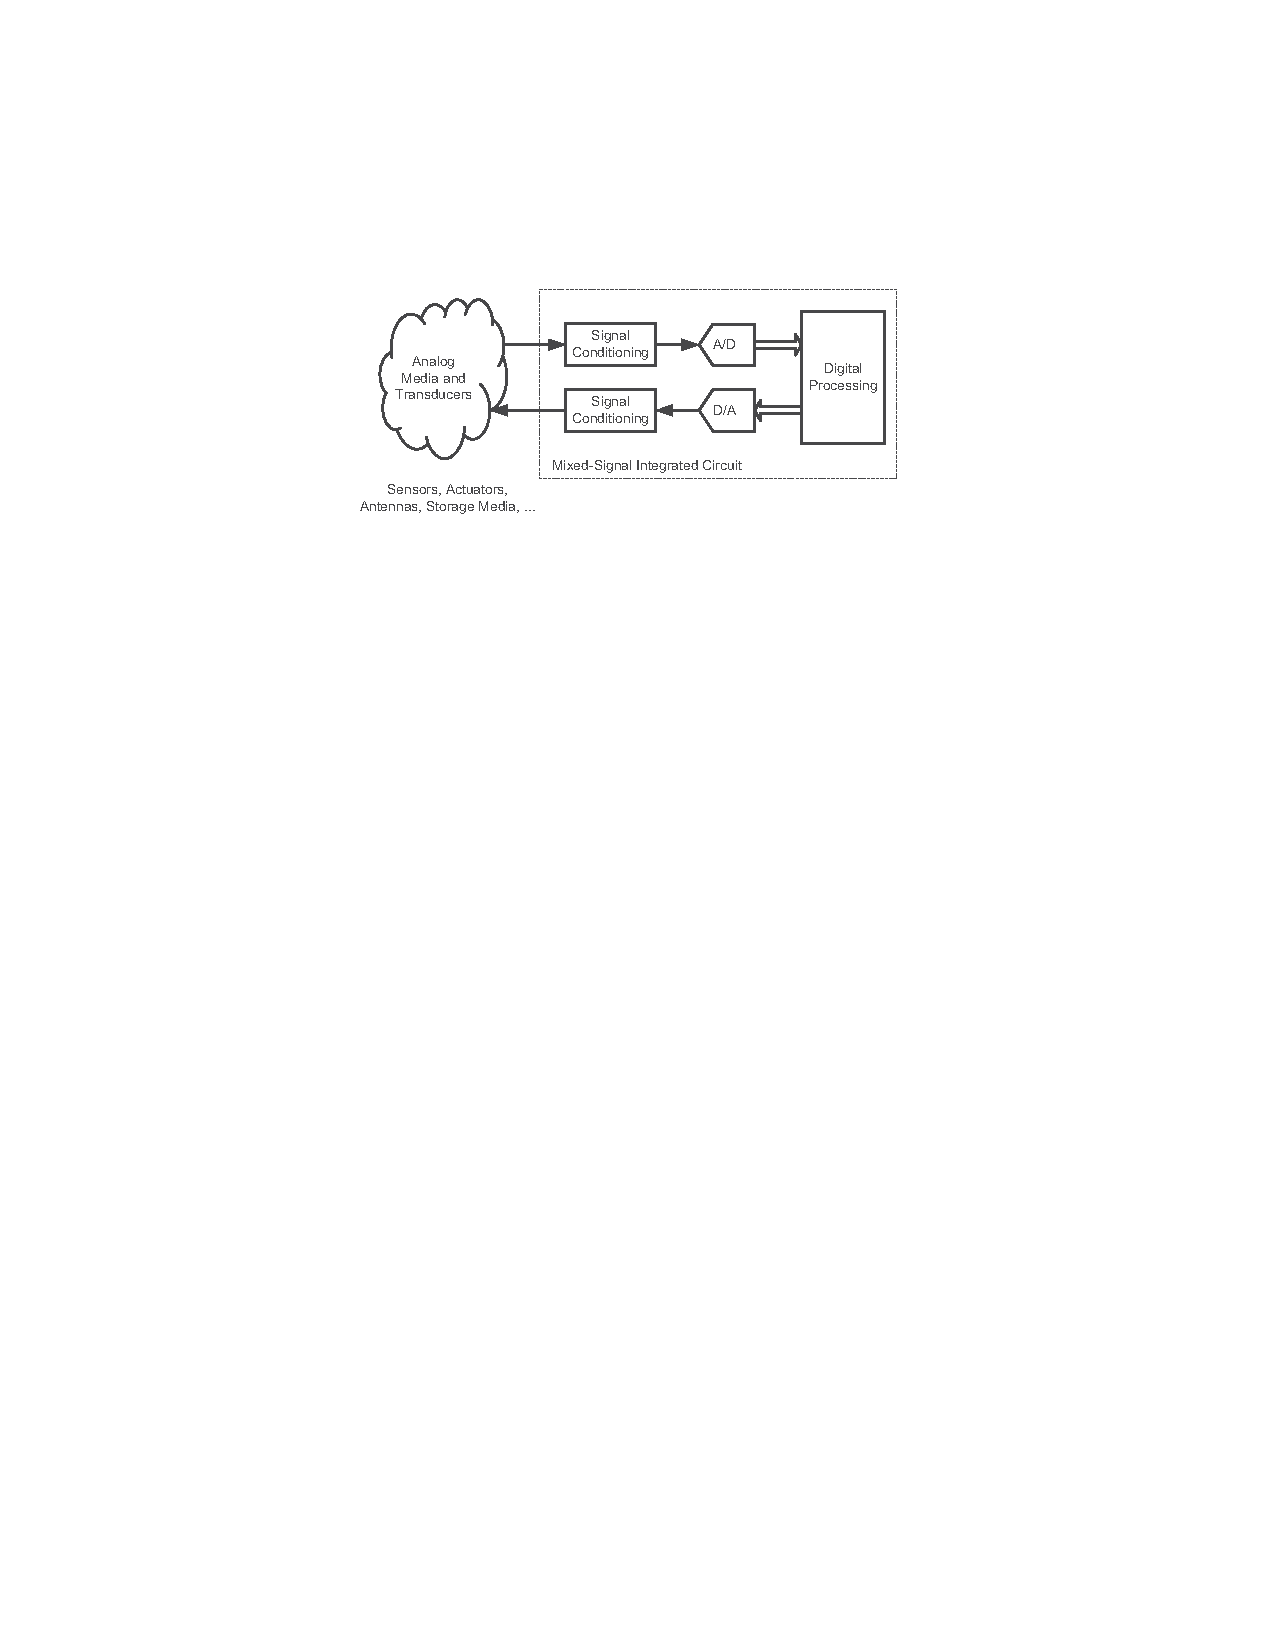
\includegraphics[width=0.5\textwidth,height=\textheight]{contents/chapter1/images/pdf/figure1.1.pdf}

}

\caption{\label{fig-1.1}Block diagram of a mixed-signal system.}

\end{figure}%

\section{Mixed-Signal Integrated
Circuits}\label{mixed-signal-integrated-circuits}

Figure~\ref{fig-1.1} shows a generic diagram of a mixed-signal system,
incorporating a mixed-signal integrated circuit. To the left of this
diagram are the transducers and media that represent the sources and
sinks of the information processed by the system. Examples of input
transducers include microphones or photodiodes used to receive
communication signals from an optical fiber. Likewise, the output of the
system may drive an antenna for radio-frequency communication or a
mechanical actuator that controls the zoom of a digital camera. At the
boundary between the media and transducers are typically signal
conditioning circuits that translate the incoming and outgoing signals
to the proper signal strength and physical format. For instance, an
amplifier is usually needed to increase the strength of the receive
signal from a radio antenna, so that it can be more easily processed by
the subsequent system components. In most systems, the signal
conditioning circuitry interfaces to analog-to-digital and
digital-to-analog converters, which provide the link between analog
quantities and their digital representation in the computing back-end of
the system.

\subsection{Example: Single-Chip Radio}\label{example-single-chip-radio}

The block diagram of a modern mixed-signal integrated circuit is shown
in Figure~\ref{fig-1.2} (see Reference 1). This design incorporates most
of the circuitry needed to realize a modern cellular phone. For
instance, it contains a front-end low-noise amplifier (LNA) to condition
the incoming antenna signal. The amplified signal is subsequently
frequency shifted, converted into digital format and fed into a digital
processor. Even though the block diagram in Figure~\ref{fig-1.2} looks
quite complex, all of its elements can be mapped into one of the blocks
of the generic diagram of Figure~\ref{fig-1.1}.

\begin{figure}

\centering{

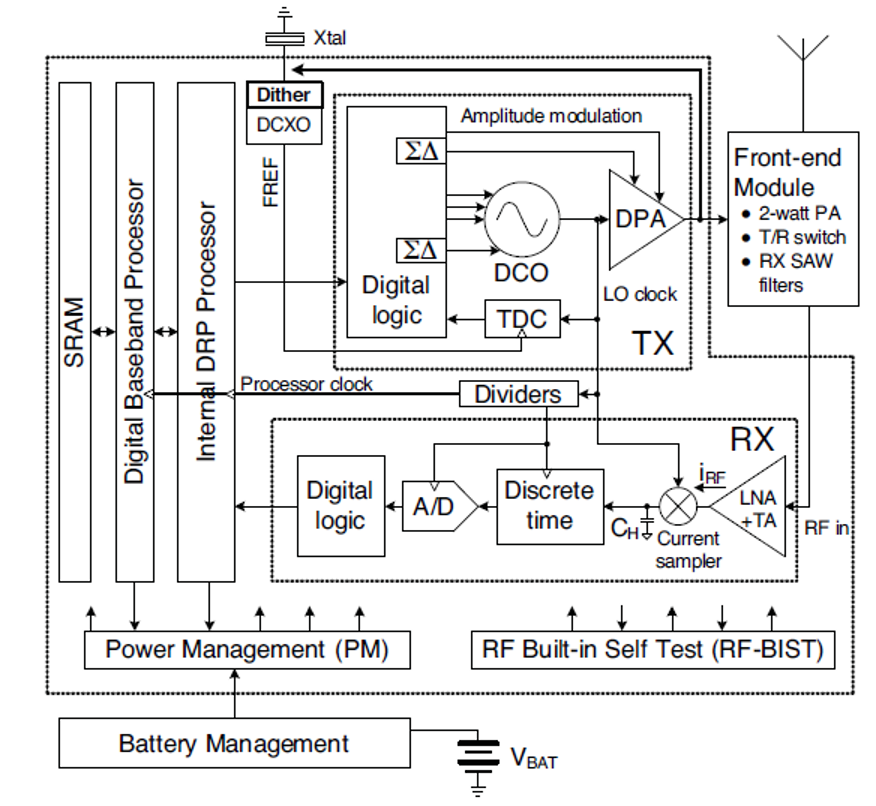
\includegraphics[width=0.5\textwidth,height=\textheight]{contents/chapter1/images/pdf/figure1.2.pdf}

}

\caption{\label{fig-1.2}Block diagram of a single-chip radio (Reference
1).}

\end{figure}%

Figure~\ref{fig-1.3} shows the chip photo of the single-chip radio, with
some of the system's key building blocks annotated. As evident from this
diagram, the digital logic dominates the area of this particular IC.
This situation is not uncommon in modern mixed-signal ICs, not least
because the utilized digital algorithms have reached an enormous
complexity, requiring millions or tens of millions of logic gates.

\begin{figure}

\centering{

\includegraphics[width=0.5\textwidth,height=\textheight]{contents/chapter1/images/pdf/figure1.3.pdf}

}

\caption{\label{fig-1.3}Chip photo of a single-chip radio (Reference
1).}

\end{figure}%

Despite the dominance of digital logic within most systems, the analog
interface components are equally important, as they determine how and
how much information can be communicated between the physical world and
the digital processing backbone. In many cases, the performance of the
signal conditioning and data conversion circuitry ultimately determines
the performance of the overall system.

\subsection{Example: Photodiode Interface
Circuit}\label{example-photodiode-interface-circuit}

Figure~\ref{fig-1.4} shows an example of a signal conditioning circuit
that plays a critical role in fiber-optic communication systems. In such
a system, a photodiode is used to convert light intensity to electrical
current (iIN). In order to condition the signal for further processing,
the diode current is converted into a voltage (vOUT) by a so-called
\textbf{transimpedance amplifier}. This amplifier must be fast enough to
process the incoming light pulses, which often occur at frequencies of
multiple gigahertz. In addition, the amplifier must obey certain limits
on power dissipation, or the system may become impractical in terms of
heat management or power supply requirements.

\begin{figure}

\centering{

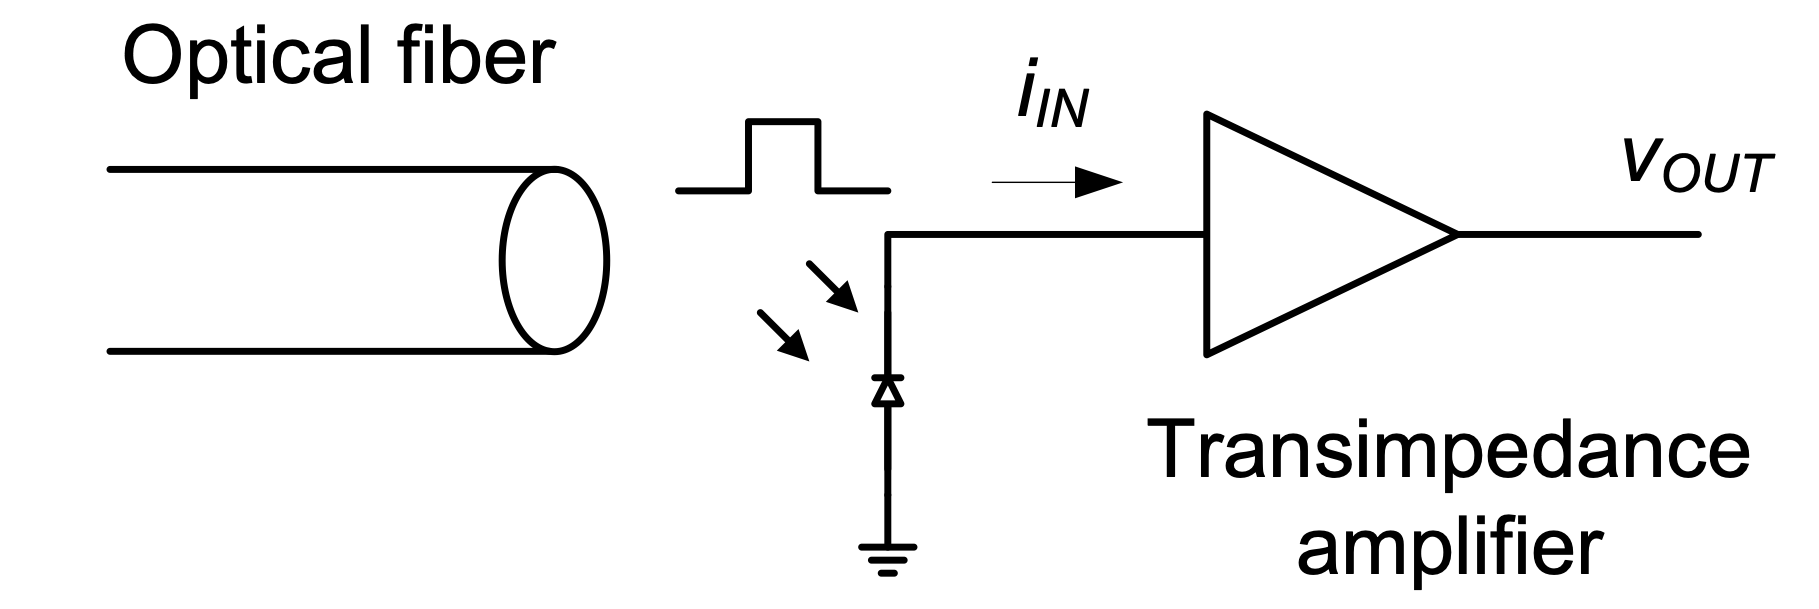
\includegraphics[width=0.5\textwidth,height=\textheight]{contents/chapter1/images/pdf/figure1.4.pdf}

}

\caption{\label{fig-1.4}Photodetector circuit for fiber-optic
communication.}

\end{figure}%

Limitations in speed and power dissipation are, in general, among the
main concerns in the interface circuitry of mixed-signal systems. Since
new products tend to demand higher performance, the analog designer is
constantly concerned with the design and optimization of system-critical
building blocks, aiming for the best possible performance that can be
achieved within the framework of the target application and process
technology.

A specific example for the circuit realization of a transimpedance
amplifier is shown in Figure~\ref{fig-1.5}. It consists of three
transistor stages, each of which serves a specific purpose and design
intent. This is true for most amplifier circuits; even though the full
schematic of a particular realization may be com- plex, it can usually
be broken up into smaller sub-blocks that are more easily understood.
Specifi- cally, for the amplifier of Figure 1-5, the experienced
designer will recognize that the circuit consists of a cascade
connection of a \textbf{common-gate}, \textbf{common-source}, and
\textbf{common-drain} stage. These sub-blocks form the basis for a large
number of analog circuits, and can be viewed as the ``atoms'' or
fundamental building blocks of analog design. In this module, you will
learn to analyze these blocks from first principles, and to reuse the
gained knowledge for the design of more complex circuits. The circuit of
Figure~\ref{fig-1.5} will be analyzed in detail in Chapter 6 of this
module, building upon the principles covered in Chapters 2--5.

\section{Managing Complexity}\label{managing-complexity}

As evident from the example of Section 1-1-1, modern integrated circuits
are highly complex and require a hierarchical approach in design and
analysis. That is, a modern integrated circuit is far too complex to be
fully understood and analyzed in a single sheet schematic at the
transistor level. Typically, a mixed-signal IC is represented by a block
diagram as the one shown in Figure~\ref{fig-1.2}. At the level of this
description, suitable specifications are derived for each block, which
may itself contain several sub-blocks. The blocks and sub-blocks are
then designed and optimized until they meet the desired target
specifications.

\begin{figure}

\centering{

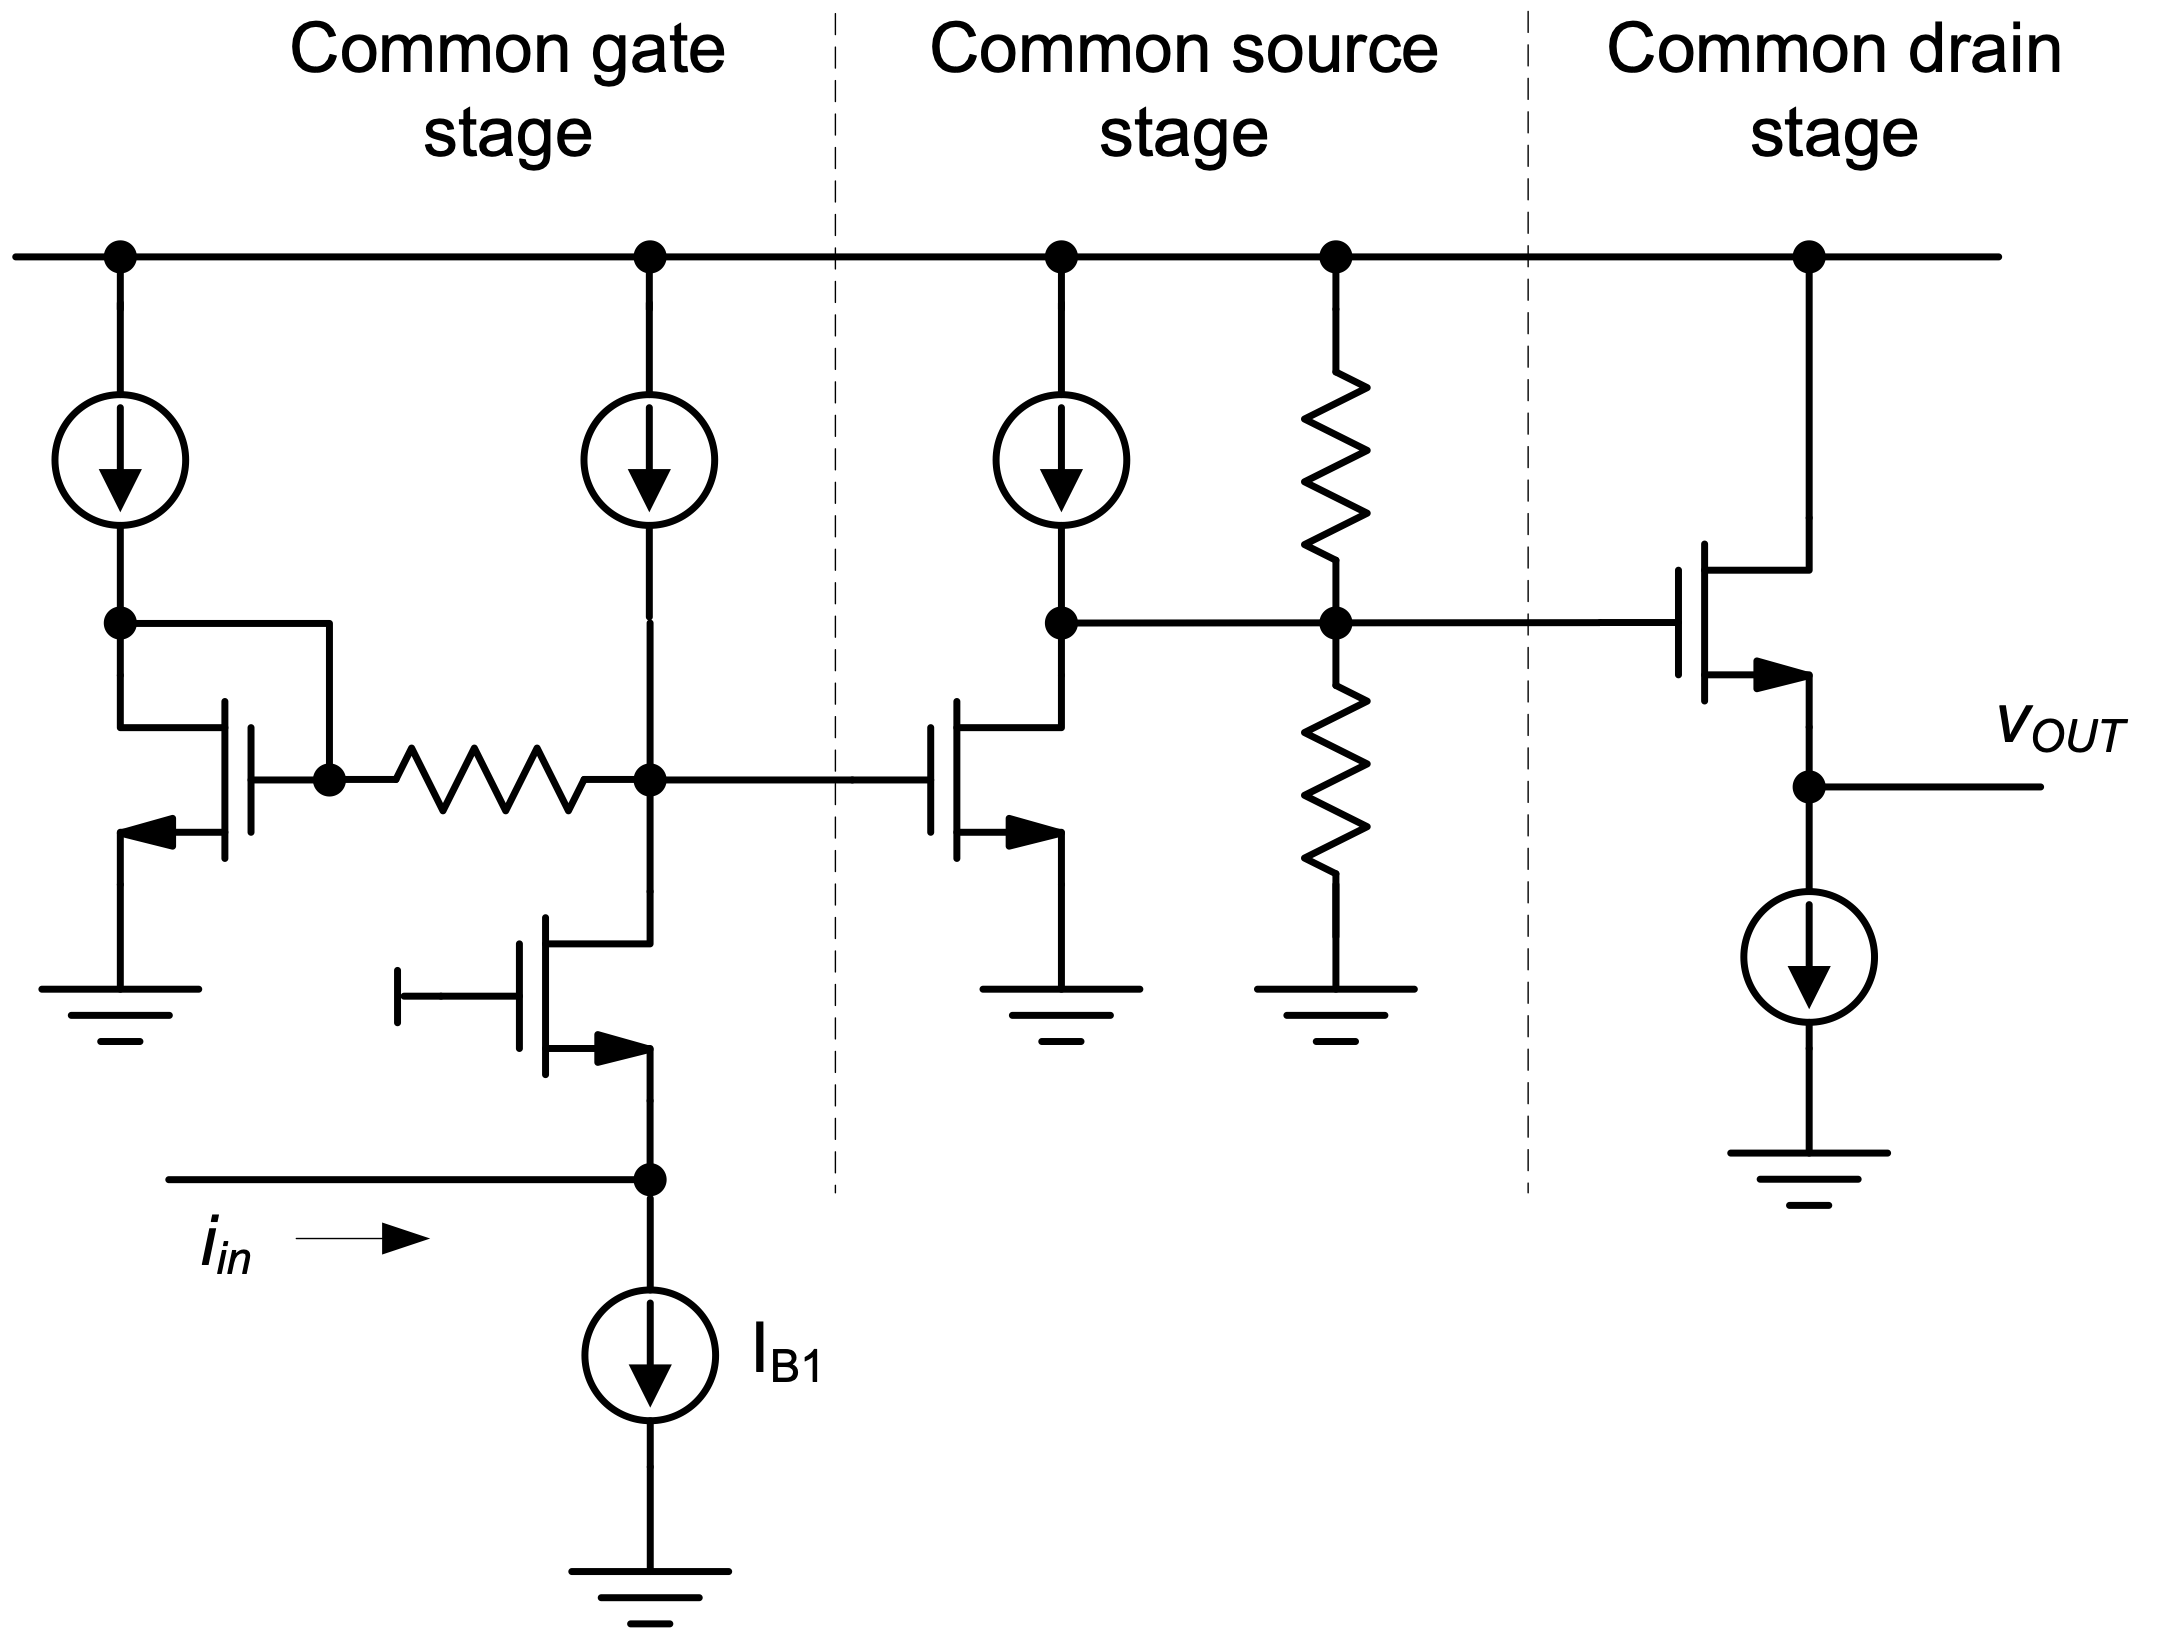
\includegraphics[width=0.5\textwidth,height=\textheight]{contents/chapter1/images/pdf/figure1.5.pdf}

}

\caption{\label{fig-1.5}Example realization of a transimpedance
amplifier.}

\end{figure}%

Figure~\ref{fig-1.6} illustrates examples of the various levels of
abstraction that come into play in the design of a modern integrated
circuit. At the highest level, the constituent elements can be
partitioned into analog and digital blocks. An example of a high-level
analog block is an analog-to-digital converter, whereas a microprocessor
is an example of a large digital block. These blocks themselves contain
smaller functional units, as, for example, operational amplifiers in the
case of an analog-to-digital converter. The operational amplifiers
themselves contain the aforementioned elementary transistor stages,
which are the main subject of this module.

\begin{figure}

\centering{

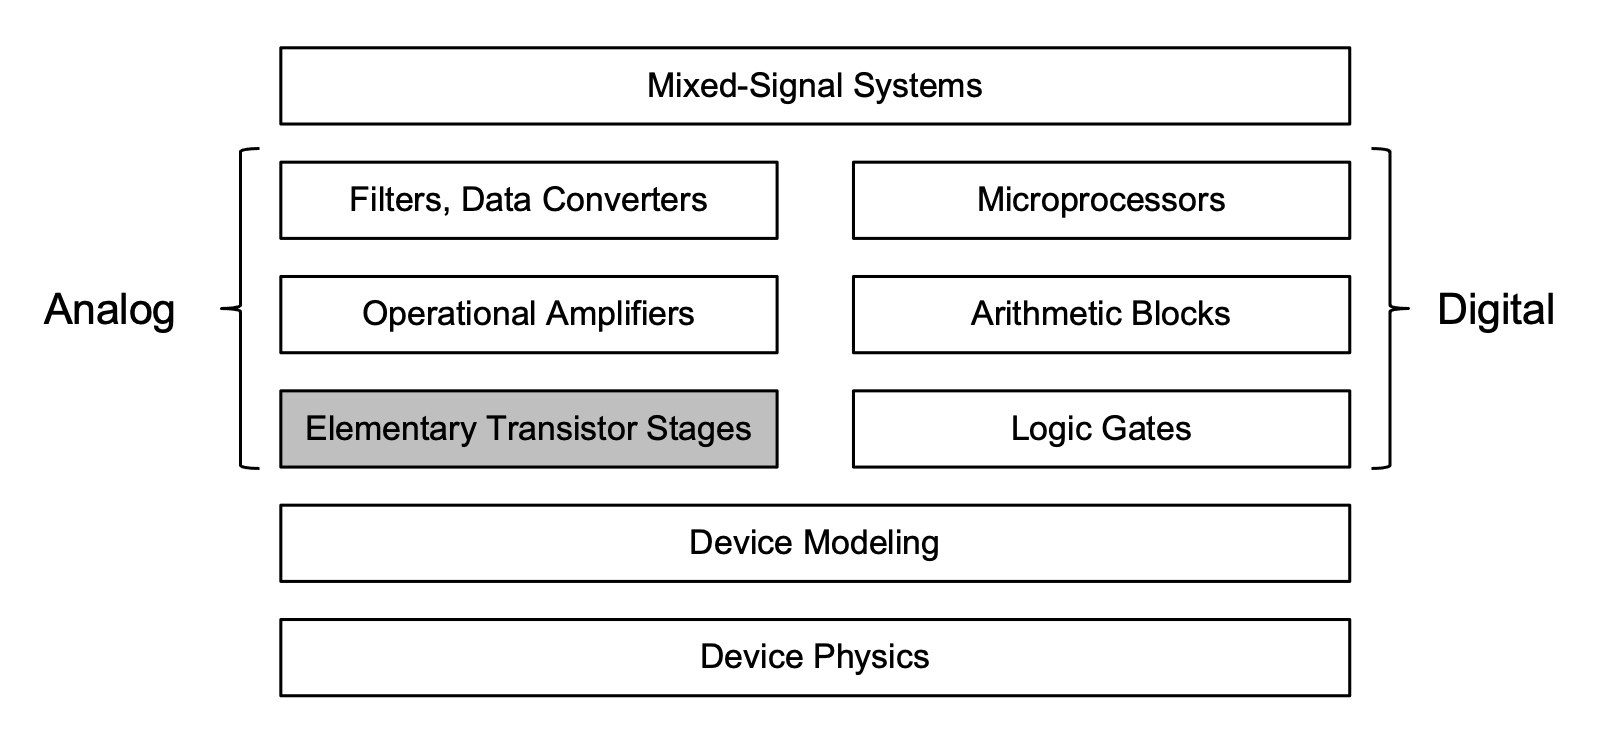
\includegraphics[width=0.5\textwidth,height=\textheight]{contents/chapter1/images/pdf/figure1.6.pdf}

}

\caption{\label{fig-1.6}Levels of abstraction in integrated circuit
design.}

\end{figure}%

Interestingly, even at the level of elementary transistor stages, is
often not possible to work with a perfect model or description of the
circuit. This is particularly so because the physical effects in the
constituent transistors are highly complex and often impossible to
capture perfectly with a tractable set of equations for hand analysis.
Therefore, making proper engineering approximations in transistor
modeling is an important aspect in maintaining a systematic design
methodology. For this particular reason, the presentation in this module
follows a ``just-in-time'' approach for the modeling of transistor
behavior. Rather than deriving a complete transistor model in an
isolated chapter (as done in most texts), we begin with only the basic
device properties and increase complexity throughout the module upon
demand, and where needed to gain further insight and accuracy. With this
approach, the reader learns to appreciate the complexity of a refined
model, and will be able to assess and track potential limitations of
working with simplified models.

\begin{figure}

\centering{

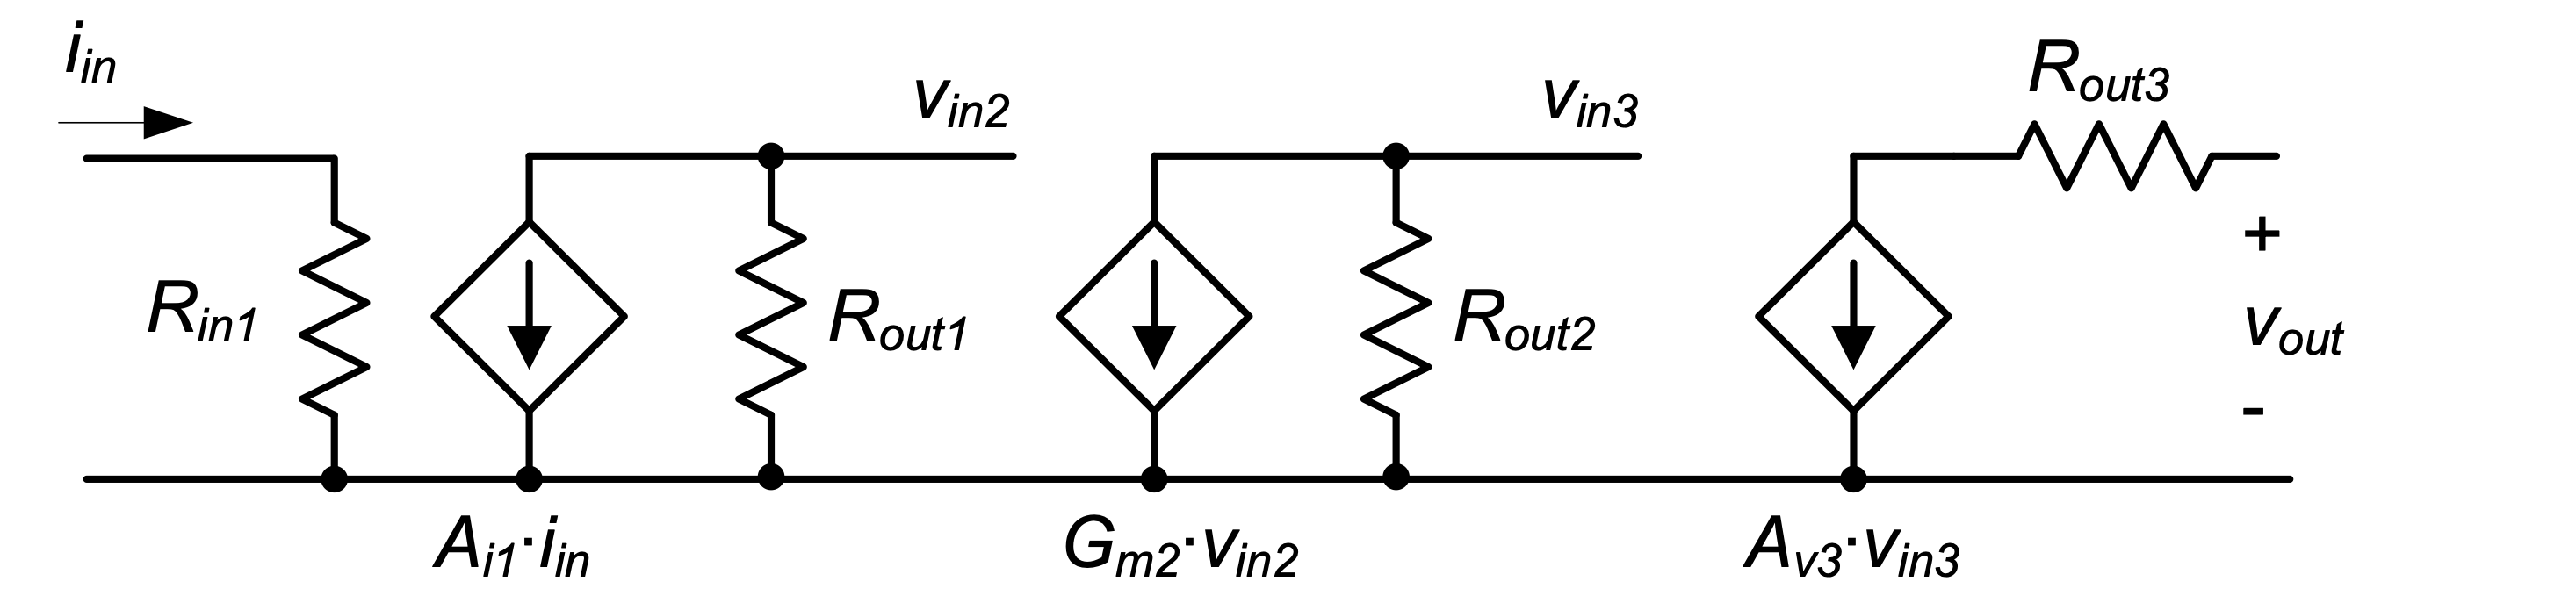
\includegraphics[width=0.5\textwidth,height=\textheight]{contents/chapter1/images/pdf/figure1.7.pdf}

}

\caption{\label{fig-1.7}Two-port model of the transimpedance amplifier
circuit in Figure~\ref{fig-1.5}.}

\end{figure}%

\section{Two-Port Abstraction for
Amplifiers}\label{two-port-abstraction-for-amplifiers}

High-level system block diagrams, such as Figure~\ref{fig-1.2} , are
typically drawn as unidirectional flowcharts and do not capture details
about the electrical behavior of each connection port and how certain
blocks may interact once they are connected. Unfortunately, electrical
signals are not unidirectional, and connecting two blocks always means
that there is some level of interaction through the voltages and
currents at the connection points.

\begin{figure}

\centering{

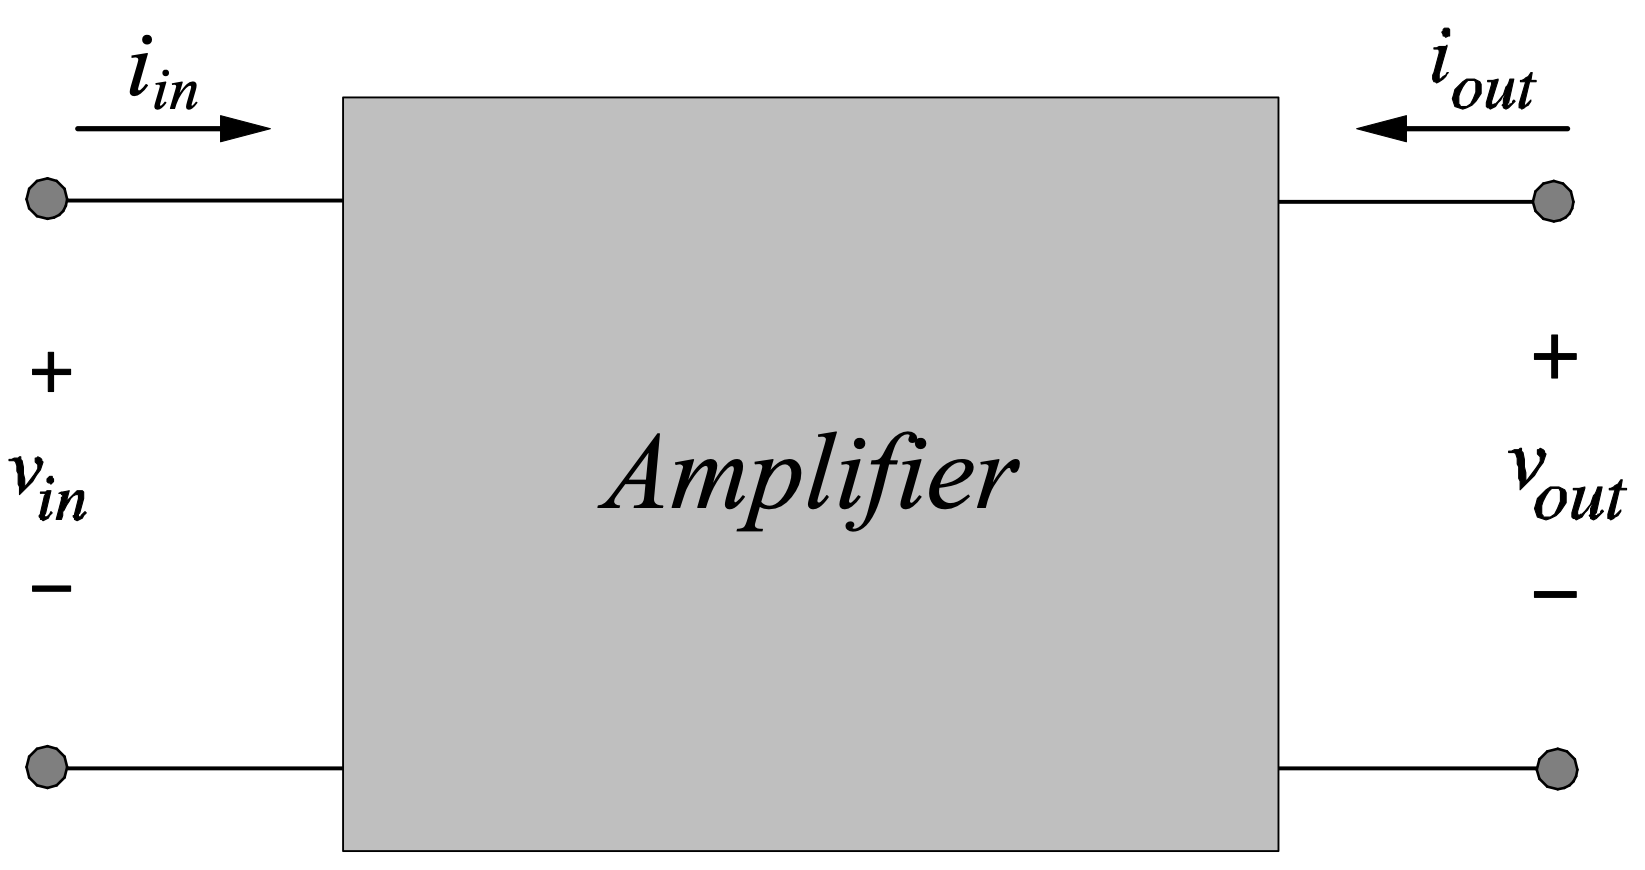
\includegraphics[width=0.5\textwidth,height=\textheight]{contents/chapter1/images/pdf/figure1.8.pdf}

}

\caption{\label{fig-1.8}General amplifier two-port.}

\end{figure}%

The commonly used linear two-port modeling abstraction for amplifiers
and amplifier stages allows the designer to take these effects into
account while maintaining a high level of abstraction. For instance, the
circuit of Figure~\ref{fig-1.5} can be approximately modeled as shown in
Figure~\ref{fig-1.7} (the details on obtaining this model are discussed
later in this module). Each stage of the overall amplifier is
represented via a simplified circuit model that captures its essential
features. Once this model is created, the interaction among stages can
be analyzed at this high level of abstraction, without requiring
detailed insight on how each stage is implemented. The two-port modeling
approach is particularly useful in the design of amplifiers, as it can
help shape the thought process on how the various stages should be
configured to optimize performance. In the following subsections, we
will review some of the basic concepts of amplifier two-port modeling
used in this module.

\subsection{Amplifier Types}\label{amplifier-types}

In this module, we model amplifier circuits as blocks that have an input
and output port, where the term ``port'' refers to a pair of terminals.
For each port, we can define input and output currents and voltages as
shown in Figure~\ref{fig-1.8}. Depending on the intended function, we
distinguish between the four possible amplifier types listed in Table
1-1. For example, an amplifier that takes an input current and amplifies
this current to produce a proportional output voltage is called a
transresistance amplifier. In this context, it is important to emphasize
that in a general practical amplifier circuit, the input and output
ports will always carry both nonzero voltages and currents, and there
exist transfer functions between all possible combinations of
input/output variables. What truly defines the type of an amplifier is
what the circuit designer deems as the main quantities of interest in
the amplifier's application.

\begin{longtable}[]{@{}
  >{\raggedright\arraybackslash}p{(\columnwidth - 4\tabcolsep) * \real{0.3973}}
  >{\raggedright\arraybackslash}p{(\columnwidth - 4\tabcolsep) * \real{0.2877}}
  >{\raggedright\arraybackslash}p{(\columnwidth - 4\tabcolsep) * \real{0.3014}}@{}}
\caption{Amplifier types.}\tabularnewline
\toprule\noalign{}
\begin{minipage}[b]{\linewidth}\raggedright
\textbf{Amplfier Type}
\end{minipage} & \begin{minipage}[b]{\linewidth}\raggedright
\textbf{Input Quantity}
\end{minipage} & \begin{minipage}[b]{\linewidth}\raggedright
\textbf{Output Quantity}
\end{minipage} \\
\midrule\noalign{}
\endfirsthead
\toprule\noalign{}
\begin{minipage}[b]{\linewidth}\raggedright
\textbf{Amplfier Type}
\end{minipage} & \begin{minipage}[b]{\linewidth}\raggedright
\textbf{Input Quantity}
\end{minipage} & \begin{minipage}[b]{\linewidth}\raggedright
\textbf{Output Quantity}
\end{minipage} \\
\midrule\noalign{}
\endhead
\bottomrule\noalign{}
\endlastfoot
Voltage Amplifier & Voltage & Voltage \\
Current Amplifier & Current & Current \\
Transconductance Amplifier & Voltage & Current \\
Transresistance Amplifier & Current & Voltage \\
\end{longtable}

Now, in order to model the inner workings of each amplifier type, we can
invoke the four corresponding two-port amplifier models shown in
Figure~\ref{fig-1.9}. Each amplifier model has an input and output
resistance (or more generally, a frequency dependent impedance) and a
controlled source to model the amplification.

\begin{itemize}
\item
  In the \textbf{voltage amplifier model}, the controlled source is a
  voltage-controlled voltage source. Ide- ally, the input resistance is
  infinite (open circuit, no current flow). The ideal output resistance
  is zero (ideal voltage source).
\item
  The \textbf{current amplifier model} has a current-con- trolled
  current source. Ideally, the input resis- tance is zero (short
  circuit, no voltage across the input port) and the output resistance
  is infinite (ideal current source).
\item
  The \textbf{transconductance amplifier model} has a volt-
  age-controlled current source. Ideally, the input resistance is
  infinite (open circuit, no current flow). The ideal output resistance
  is also infinite (ideal current source).
\item
  The \textbf{transresistance or transimpedance\footnote{The term
    transimpedance is sometimes used to refer to an amplifier that is
    primarily meant to realize a transresistance. Referring to
    ``impedance'' highlights the fact that the transfer function will
    usually be frequency-dependent.} amplifier model} has a
  current-controlled voltage source. Ideally, the input resistance is
  zero (short circuit, no voltage across the input port). The ideal out-
  put resistance is also zero (ideal voltage source).
\end{itemize}

From these four models and their ideal behavior, we note that the
two-ports containing a voltage-controlled source should ideally have
large input resistance (Rin). This minimizes the signal loss due to
resistive voltage division between the source voltage (vs) and the
control voltage (vin). In contrast, the two-ports that use a
current-controlled source should have small input resistance to minimize
the signal loss due to current division between the source current (is)
and the control current (iin). In this context, ``large'' and ``small''
refer to the value of Rin relative to the source resistance (Rs).

\begin{figure}

\centering{

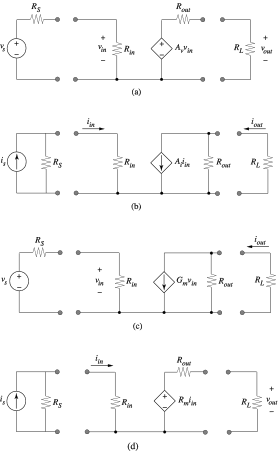
\includegraphics[width=0.5\textwidth,height=\textheight]{contents/chapter1/images/pdf/figure1.9.pdf}

}

\caption{\label{fig-1.9}Two-port amplifier models with input source and
load: (a) voltage amplifier, (b) current amplifier, (c) transconductance
amplifier, and (d) transresistance amplifier.}

\end{figure}%

On the output side, if the variable of interest is a voltage, the output
resistance (Rout) should be small so that only a small amount of the
amplified voltage is lost through the division with the load (RL).
Conversely, for a current output, the output resistance should be large
to minimize current division losses. Again, ``large'' and ``small'' are
taken as relative measures comparing Rout to RL.

Consider for example the voltage amplifier of Figure~\ref{fig-1.9}(a).
To calculate the transfer function of the overall circuit (vout/vs), the
input voltage, including its source resistance, is connected to the
input of the two-port model and the load resistance is connected to the
output. The full circuit is shown in Figure~\ref{fig-1.10}.

\begin{figure}

\centering{

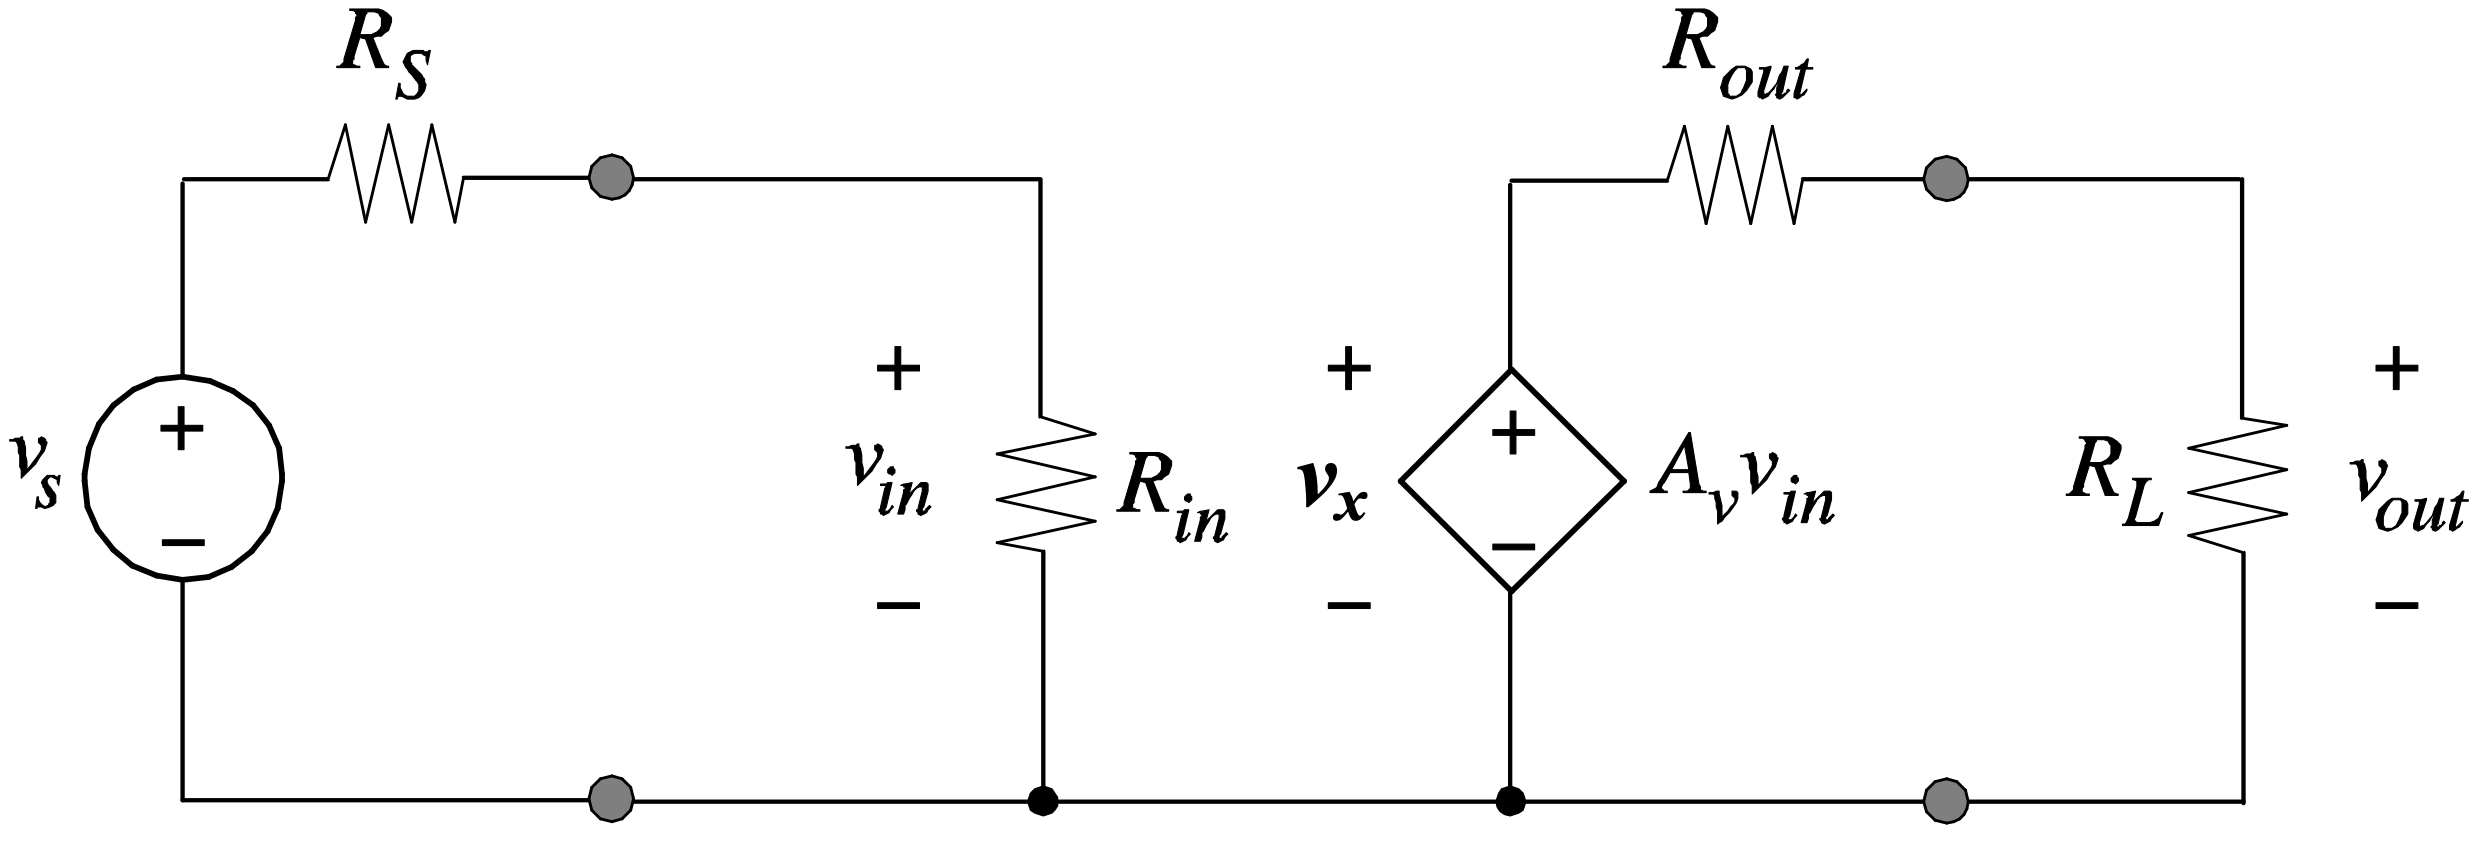
\includegraphics[width=0.5\textwidth,height=\textheight]{contents/chapter1/images/pdf/figure1.10.pdf}

}

\caption{\label{fig-1.10}Voltage amplifier with connected source and
load resistances.}

\end{figure}%

Applying the voltage divider rule at the input and output of the circuit
gives

\begin{equation}\phantomsection\label{eq-1.1}{
\frac{v_{out}}{v_s} = \Bigl(\frac{v_{in}}{v_s}\Bigr) \cdot A_v \cdot \Bigl(\frac{v_{out}}{v_x}\Bigr) = \Bigl(\frac{R_{in}}{R_{in} + R_s}\Bigr) \cdot A_v \cdot \Bigl(\frac{R_{L}}{R_{L} + R_{out}}\Bigr)
}\end{equation}

As we can see from this expression, the overall voltage gain is
maximized when the amplifier has a large input resistance (relative to
Rs) and a small output resistance (relative to RL). For the ideal case
of infinite input resistance and zero output resistance, vout/vs becomes
equal to Av.

For the sake of compact notation, we will often want to use a symbol for
the overall circuit gain. The notation used in this module uses primed
variables to distinguish between the gain of the controlled source and
the gain of the overall amplifier circuit. For example, for the
above-discussed voltage amplifier we define A′v = v out ⁄ v s . This
notation is meant to emphasize the connection between the two symbols.
A′v is usually smaller than Av, but can approach Av for ideal source and
load configurations.

\textbf{Example 1-1: Transfer Function Transconductance Amplifier.}

For the transconductance amplifier circuit in Figure Ex1-1, calculate
the overall transconductance G′m = i out ⁄ v s .

\begin{figure}

\centering{

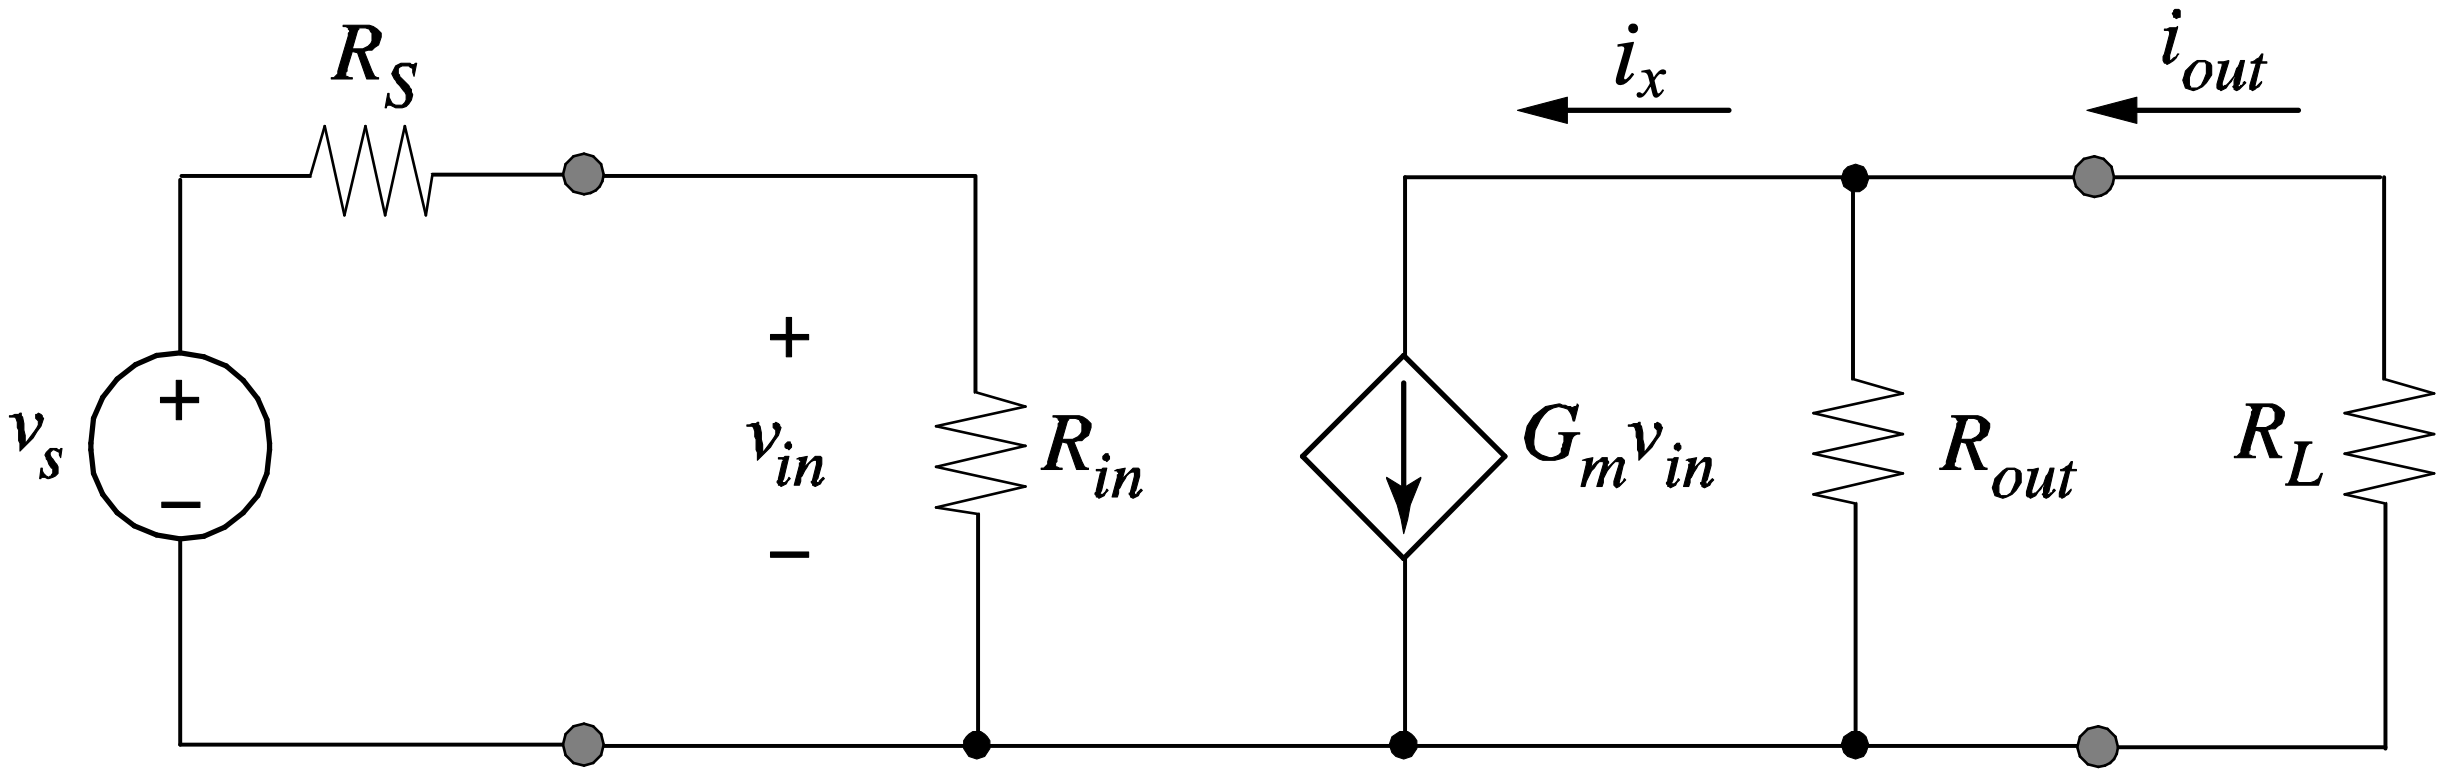
\includegraphics[width=0.5\textwidth,height=\textheight]{contents/chapter1/images/pdf/figure-ex-1.1.pdf}

}

\caption{\label{fig-ex-1.1}\textbf{Figure Ex 1-1}}

\end{figure}%

\textbf{SOLUTION}

Applying the voltage divider rule at the input and the current divider
rule at the output yields the following result:

\[
G'_m = \frac{i_{out}}{v_s} = \Bigl(\frac{v_{in}}{v_s}\Bigr) \cdot G_m \cdot \Bigl(\frac{i_{out}}{i_x}\Bigr) =  \Bigl(\frac{R_{in}}{R_{in} + R_s}\Bigr) \cdot G_m \cdot \Bigl(\frac{R_{L}}{R_{L} + R_{out}}\Bigr)
\]

Thus, the overall transconductance gain is maximized when the amplifier
has a large input resistance (relative to Rs) and a large output
resistance (relative to RL). For the ideal case of infinite input and
output resistances, G′m becomes equal to Gm.

As a final remark for this sub-section, it is important to recognize
that all of the models in Figure~\ref{fig-1.9} can be used
interchangeability to describe the exact same electrical behavior (see
Problem P1-1). For instance, a voltage amplifier model can be converted
into a transconductance amplifier model by applying a Thevénin to Norton
transformation for the controlled source.

A corollary to this equivalence is that we can for example use a
transconductance amplifier model to describe a voltage amplifier
circuit. This is illustrated through the circuit of
Figure~\ref{fig-1.10}, which is electrically equivalent to that of
Figure~\ref{fig-1.10} (see Problem P1-2). Note that the output is taken
as the voltage across the output port instead of the output current;
this indicates that the circuit is viewed as a voltage amplifier. Just
as in the original circuit of Figure~\ref{fig-1.10}, we require a large
input resistance and small output resistance for this circuit to
maximize the overall voltage gain.

The choice of amplifier model depends on several factors. At first
glance, it seems natural to model each amplifier type using its
``native'' model that directly corresponds to the intended function. For
example, we could always describe a voltage amplifier using the
corresponding voltage amplifier model that contains a voltage controlled
voltage source. However, as we shall see throughout this module, it is
sometimes more convenient to align the amplifier model with the physical
amplification mechanism or a structural feature of the underlying
transistor circuit. For instance, the common-source voltage amplifier
discussed in Chapter 2 naturally invokes a transconductance-based model
due to the physical model of the employed transistor.

\subsection{Unilateral versus Bilateral
Two-Ports}\label{unilateral-versus-bilateral-two-ports}

All of the two-port models shown in Figure~\ref{fig-1.9} are called
\textbf{unilateral}, because they can only propagate a signal from the
input port to the output port and not the other way around. For
instance, injecting a current into the output port of the current
amplifier of (\citeproc{ref-fig1.9}{\textbf{fig1.9?}})(b) will not
induce a current at the input port. Unfortunately, many practical
transistor circuits are not unilateral, and exhibit \textbf{bilateral}
behavior when analyzed in detail, and especially at high frequencies.

\begin{figure}

\centering{

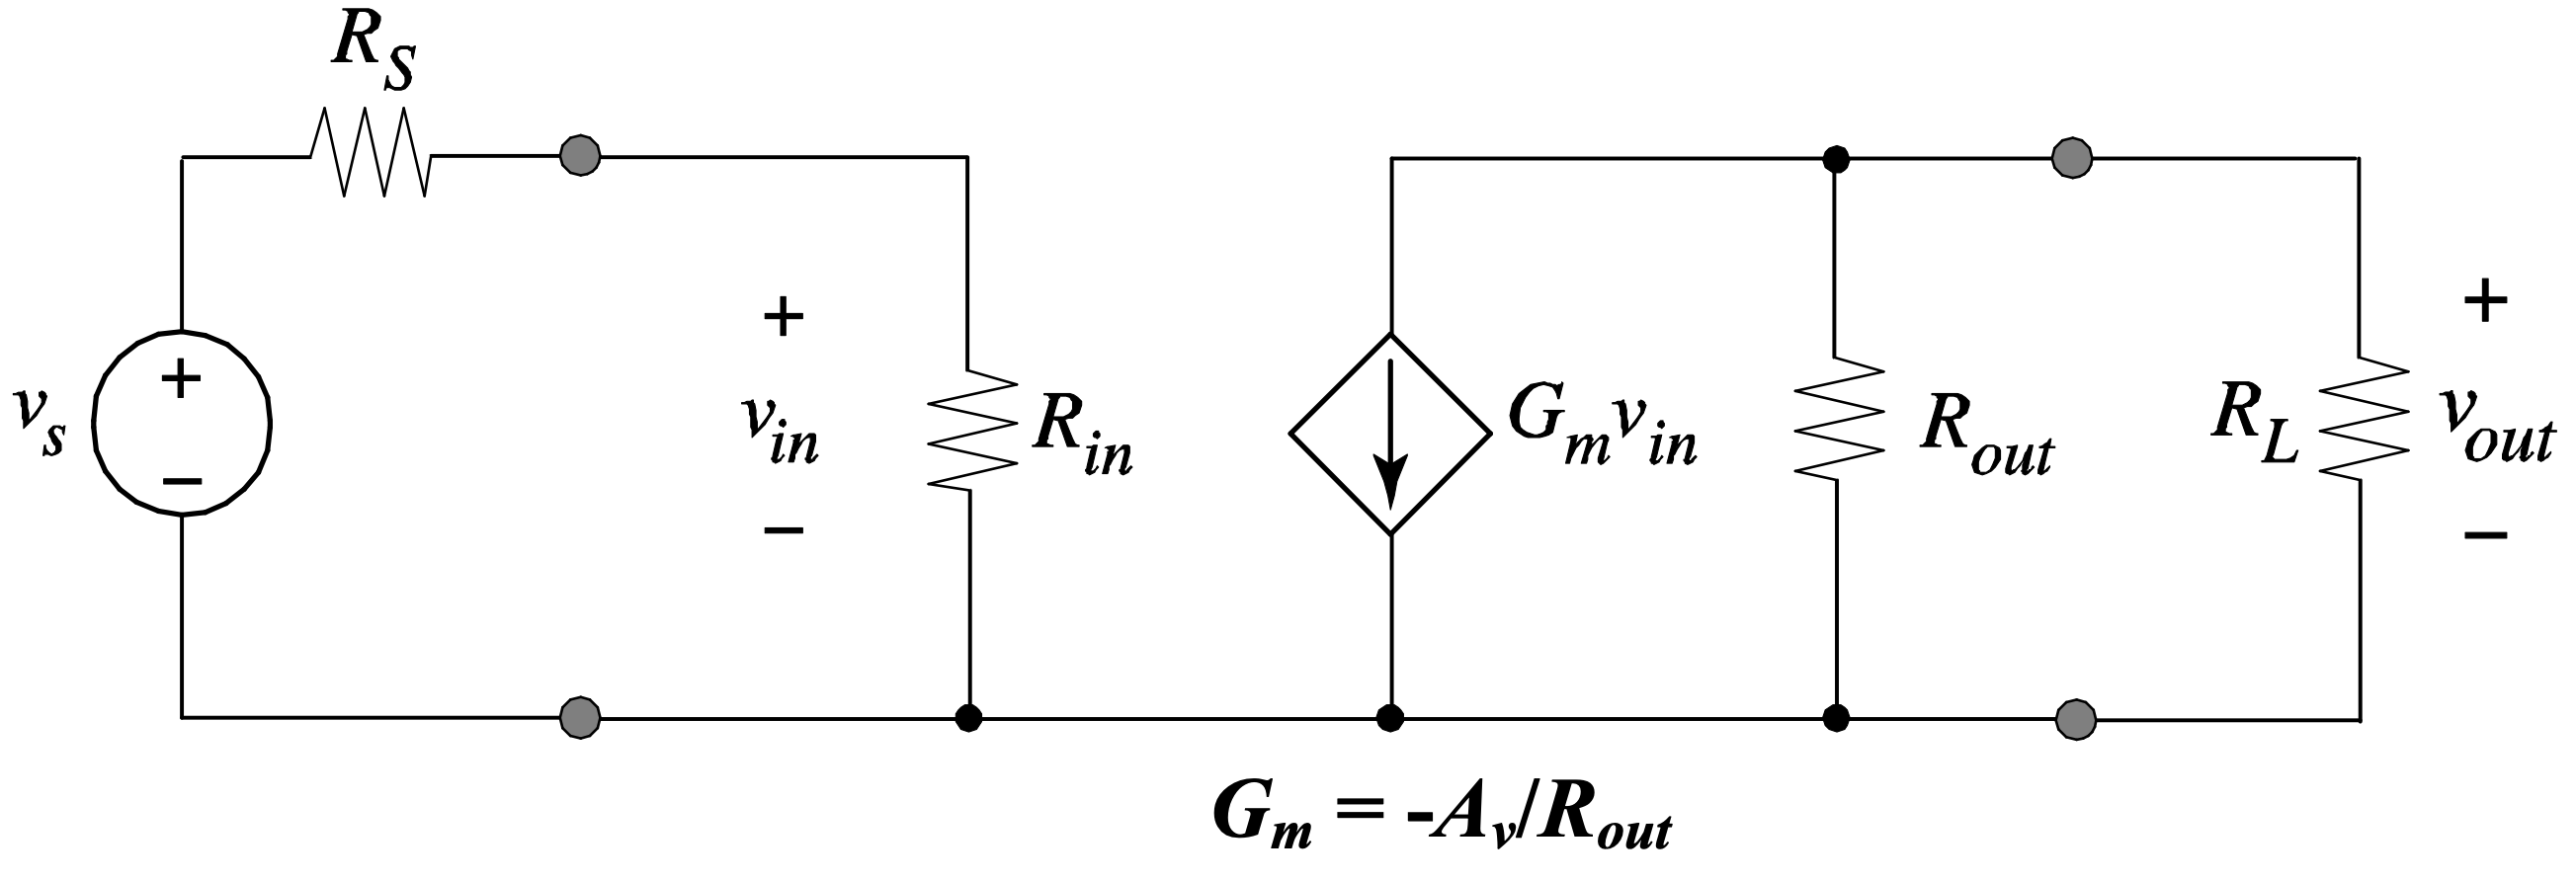
\includegraphics[width=0.5\textwidth,height=\textheight]{contents/chapter1/images/pdf/figure1.11.pdf}

}

\caption{\label{fig-1.11}Voltage amplifier with an underlying
transconductance amplifier model}

\end{figure}%

\begin{figure}

\centering{

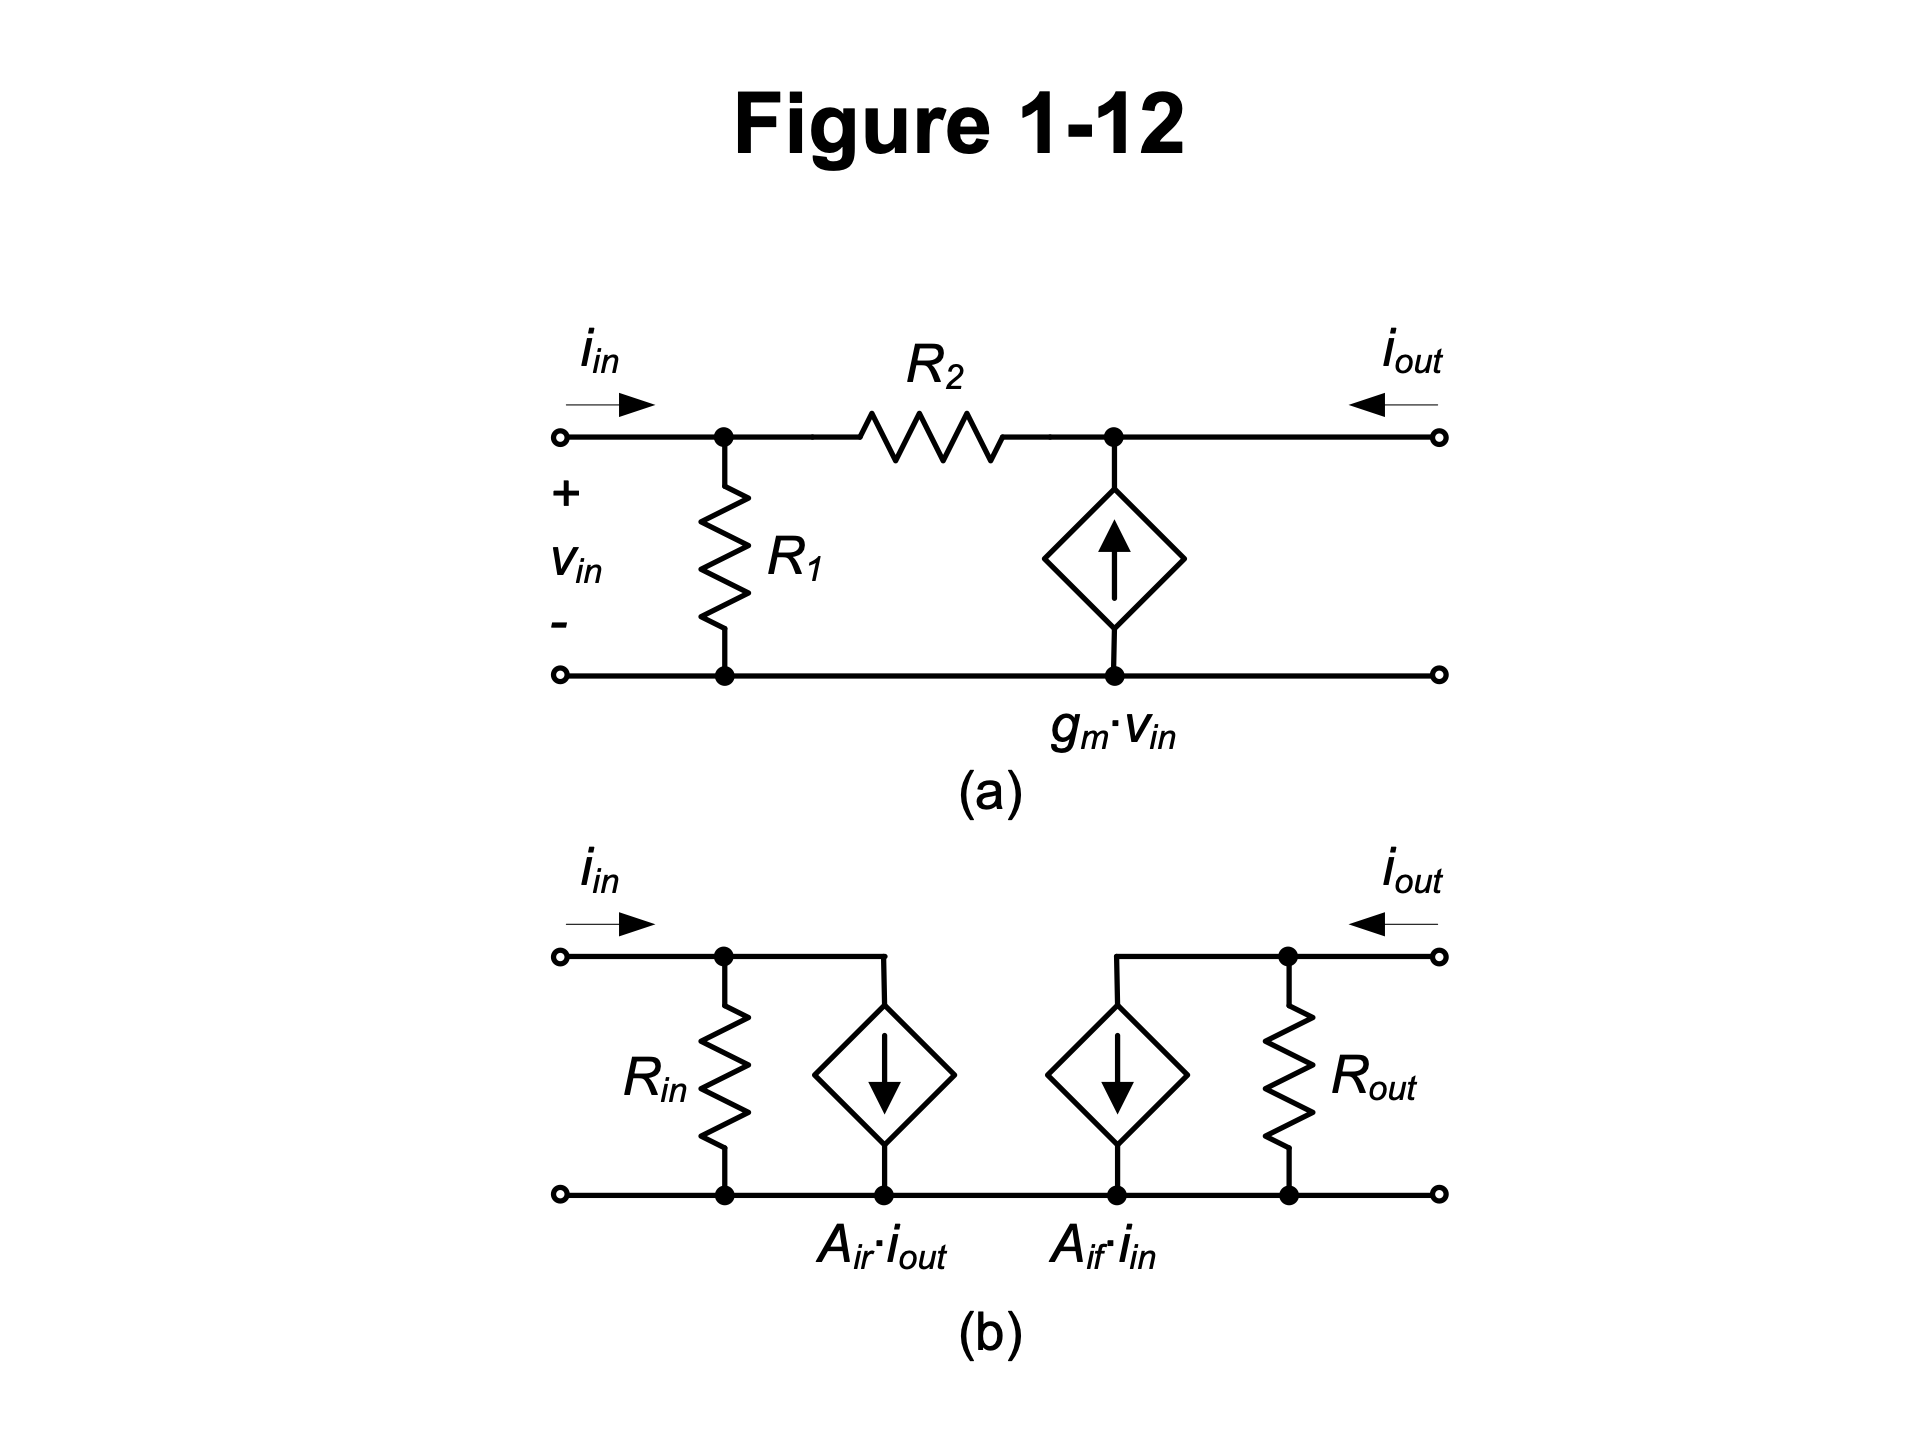
\includegraphics[width=0.5\textwidth,height=\textheight]{contents/chapter1/images/pdf/figure1.12.pdf}

}

\caption{\label{fig-1.12}(a) Example of a bilateral current amplifier.
(b) Corresponding bilateral current amplifier two-port model.}

\end{figure}%

An example of a bilateral current amplifier is shown
Figure~\ref{fig-1.12}(a). Note that in this circuit, resistor R2 couples
the input and output networks and it can therefore transfer currents in
both directions. Consequently, the unilateral model of
Figure~\ref{fig-1.9}(b) cannot perfectly represent this circuit. When it
is desired to capture the bilateral behavior, the two-port model in
Figure Figure~\ref{fig-1.12}(b) could be employed in principle. Here,
the controlled source Air models the reverse current transfer from the
output back to the input. Alternatively, one could employ other
bilateral and more general two-port models based on admittance
parameters (Y), impedance parameters (Z), and hybrid or inverse-hybrid
parameters (H or G); see advanced circuit design texts such as Reference
2. These models are particularly useful when reverse transmission (i.e.,
feedback from the output to the input) is incorporated in the circuit as
part of the intended design.

There are two reasons why we will work exclusively with unilateral
two-port approximations in this module. First, the circuits considered
are designed primarily to implement forward gain rather than reverse
gain; feedback circuits are not treated in this module. For example,
referring to the model of Figure~\ref{fig-1.12}(b), the reverse gain Air
will be negligibly small in any current amplifier circuit that we will
consider. Second, a clear drawback of working with bilateral two-port
models would be a significant increase in analysis complexity. As we
have seen in Example 1-1, the overall transfer function of a unilateral
two-port circuit can be written by applying simple voltage and current
divider rules. This also extends to cascade connections of multiple
two-ports. For example, the overall transfer function of the circuit in
Figure~\ref{fig-1.7} is easily written by inspection, without requiring
extensive algebra. With reverse transmission included, the transfer
function analysis will generally require solving a linear system of
equations. In light of the fact that we do not intend to design circuits
in this module that have significant reverse transmission, this increase
in complexity is not welcome, and would also hinder us from developing
intuition from inspection-driven analysis.

\subsection{Construction of Unilateral Two-Port
Models}\label{construction-of-unilateral-two-port-models}

We will now describe the general procedures to calculate the controlled
sources, as well as the input and output resistances, for the unilateral
two-port models of Figure~\ref{fig-1.9}. The approach is based on
applying test voltages and currents to find the desired model
parameters.

The most important parameter of any amplifier circuit is its gain. To
identify the gain parameters for the models of
Figure~\ref{fig-1.9}(a)-(d), we apply the tests shown in
Figure~\ref{fig-1.13}(a)-(d), respectively.

\begin{itemize}
\item
  To calculate the gain term Av of a voltage amplifier model, we apply a
  test voltage at the input with zero source resistance and measure the
  open-circuit output voltage. Av = voc/vt is therefore also called the
  \textbf{open-circuit voltage gain}.
\item
  To calculate the gain term Ai of a current amplifier model, we apply a
  test current at the input with infinite source resistance and measure
  the short-circuit output current. Ai = isc/it is therefore also called
  the \textbf{short-circuit current gain}.
\item
  To calculate the gain term Gm of a transconductance amplifier model,
  we apply a test voltage at the input with zero source resistance and
  measure the short-circuit output current to find Gm = isc/vt.
\item
  To calculate the gain term Rm of a transresistance amplifier model, we
  apply a test current at the input with infinite source resistance and
  measure the open-circuit output voltage to find Rm = voc/it.
\end{itemize}

\begin{figure}

\centering{

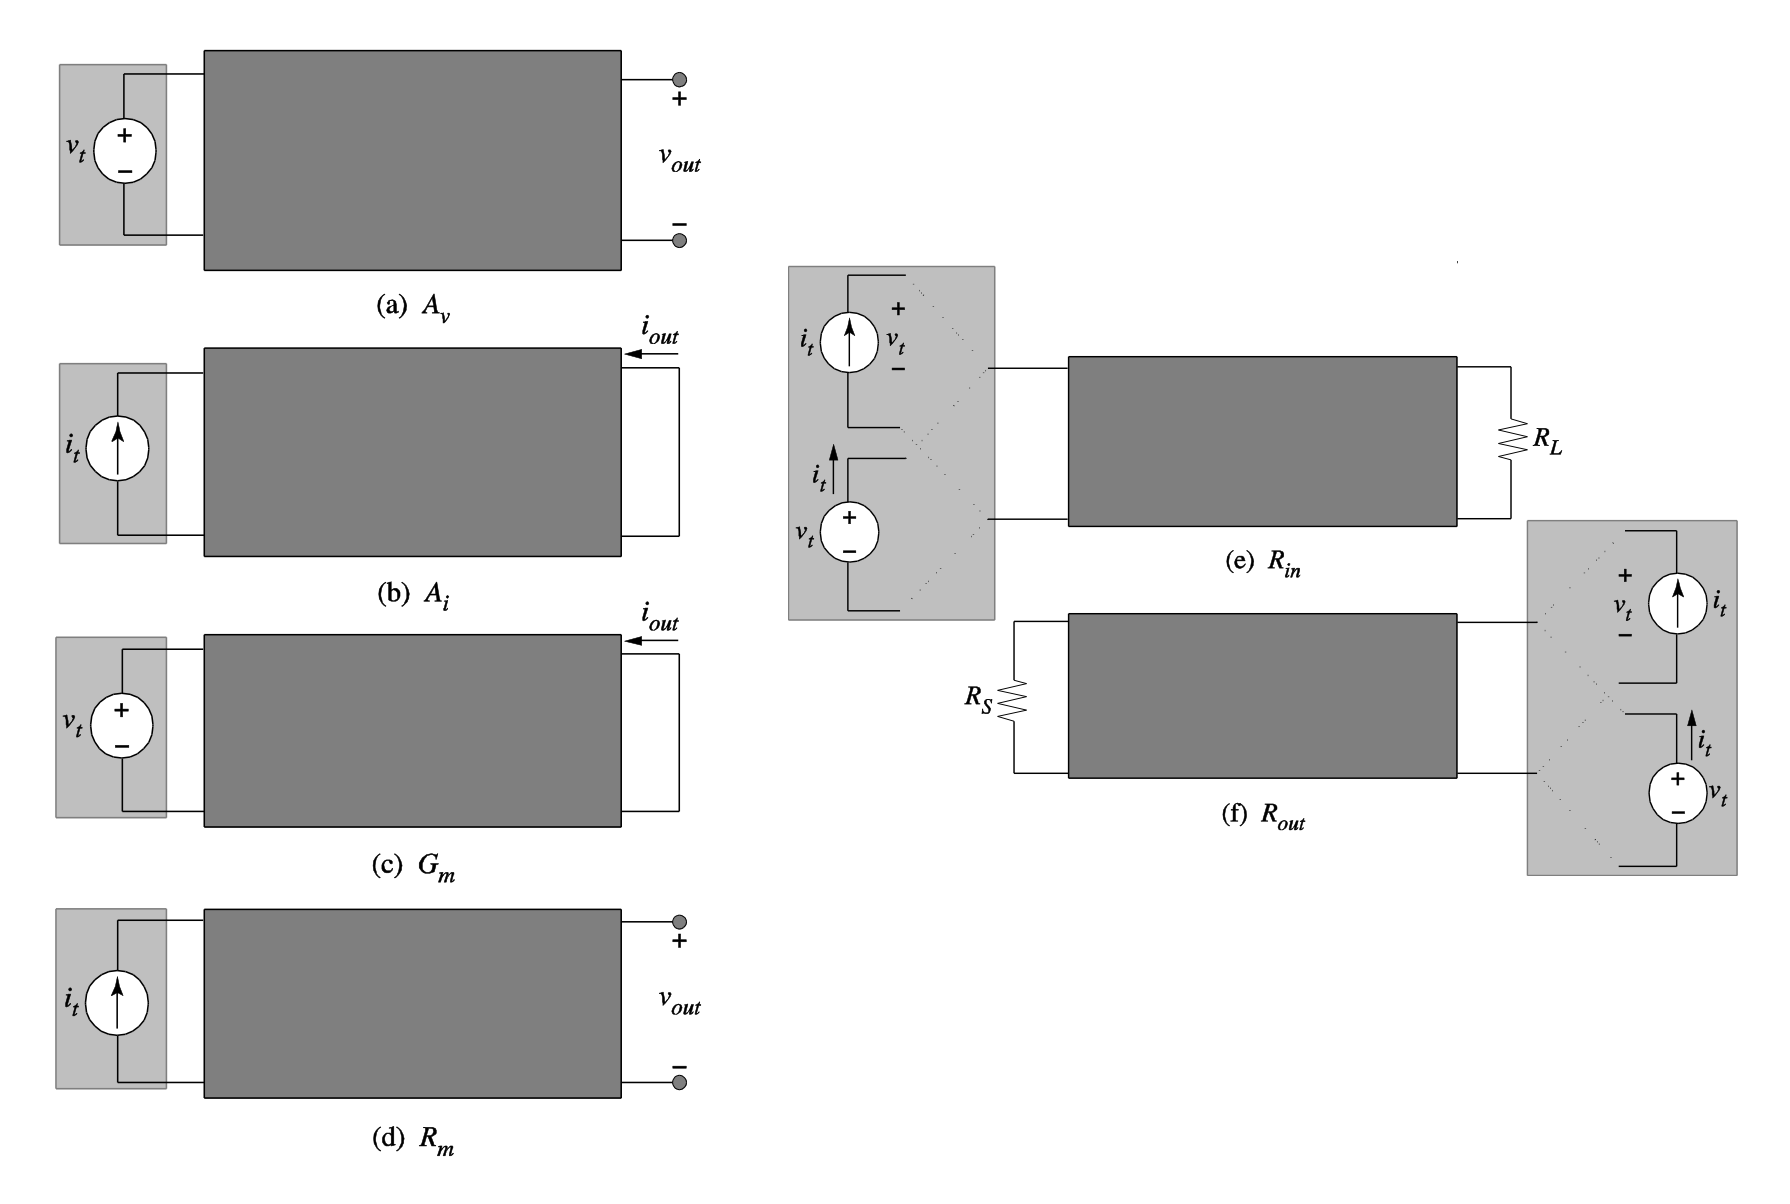
\includegraphics[width=0.5\textwidth,height=\textheight]{contents/chapter1/images/pdf/figure1.13.pdf}

}

\caption{\label{fig-1.13}Method to calculate two-port amplifier model
parameters: (a) voltage gain Av, (b) current gain Ai, (c)
transconductance Gm, (d) transresistance Rm, (e) input resistance Rin,
and (f) output resistance Rout.}

\end{figure}%

The rationale behind these tests can be understood by considering, for
example, the case of the voltage amplifier model of
Figure~\ref{fig-1.9}(a). When driven with an ideal voltage source, the
effect of any resistance at the input port is eliminated, and the
controlled source is directly stimulated by the applied test source
(without any voltage division). Likewise, by measuring the resulting
output voltage open-circuited, any resistance in series with the
controlled source has no effect and the measurement therefore accurately
extracts the parameter Av. Similar explanations apply to the test cases
for the remaining amplifier models.

The test setup for extracting the input and output resistances for all
amplifier models is shown in Figure~\ref{fig-1.13}(e), and (f),
respectively.

\begin{itemize}
\item
  To calculate the \textbf{input resistance} Rin we apply a test voltage
  and measure the current coming from the test source, or apply a test
  current and mea- sure the voltage across the test source. In this
  test, the load resistance (RL) must be connected to the output port as
  shown in Figure~\ref{fig-1.13}(e).
\item
  To calculate the \textbf{output resistance} Rout, we apply either a
  test voltage or a test current source at the output port and measure
  the respective current or voltage from the source. Here, the input
  source must be set equal to zero. This means that input voltage
  sources are shorted and input current sources are open-circuited. Only
  the source resistance (RS) is left across the input terminals as shown
  in Figure~\ref{fig-1.13}(f).
\end{itemize}

The above procedures extract the input and output resistances perfectly
and without any approximations, even if the circuit is bilateral. As we
shall see through the examples below, Rin and Rout do not depend on RL
and RS, respectively, in a perfectly unilateral amplifier. However, this
is not the case in a bilateral amplifier, and therefore the general
procedure includes RL and RS in the test setup.

In summary, the above procedures for measuring unilateral two-port model
parameters aim at finding the best possible unilateral representation of
an arbitrary amplifier circuit, which itself may or may not be
unilateral. The obtained models are approximate when the amplifier is
bilateral, since they do not include a controlled source that captures
reverse transmission from the output back to the input. In most cases
considered in this module, the reverse transmission term is negligible.
Exceptions will be highlighted and treated as appropriate.

\textbf{Example 1-2: Two-Port Model Calculations for a Unilateral
Amplifier}

For the transconductance amplifier in Figure Ex1-2A, calculate the
following two-port model parameters: the transconductance Gm, the input
resistance Rin, and the output resistance Rout. Also, compute the
overall transfer function G′m = i out ⁄ v s.

\begin{figure}

\centering{

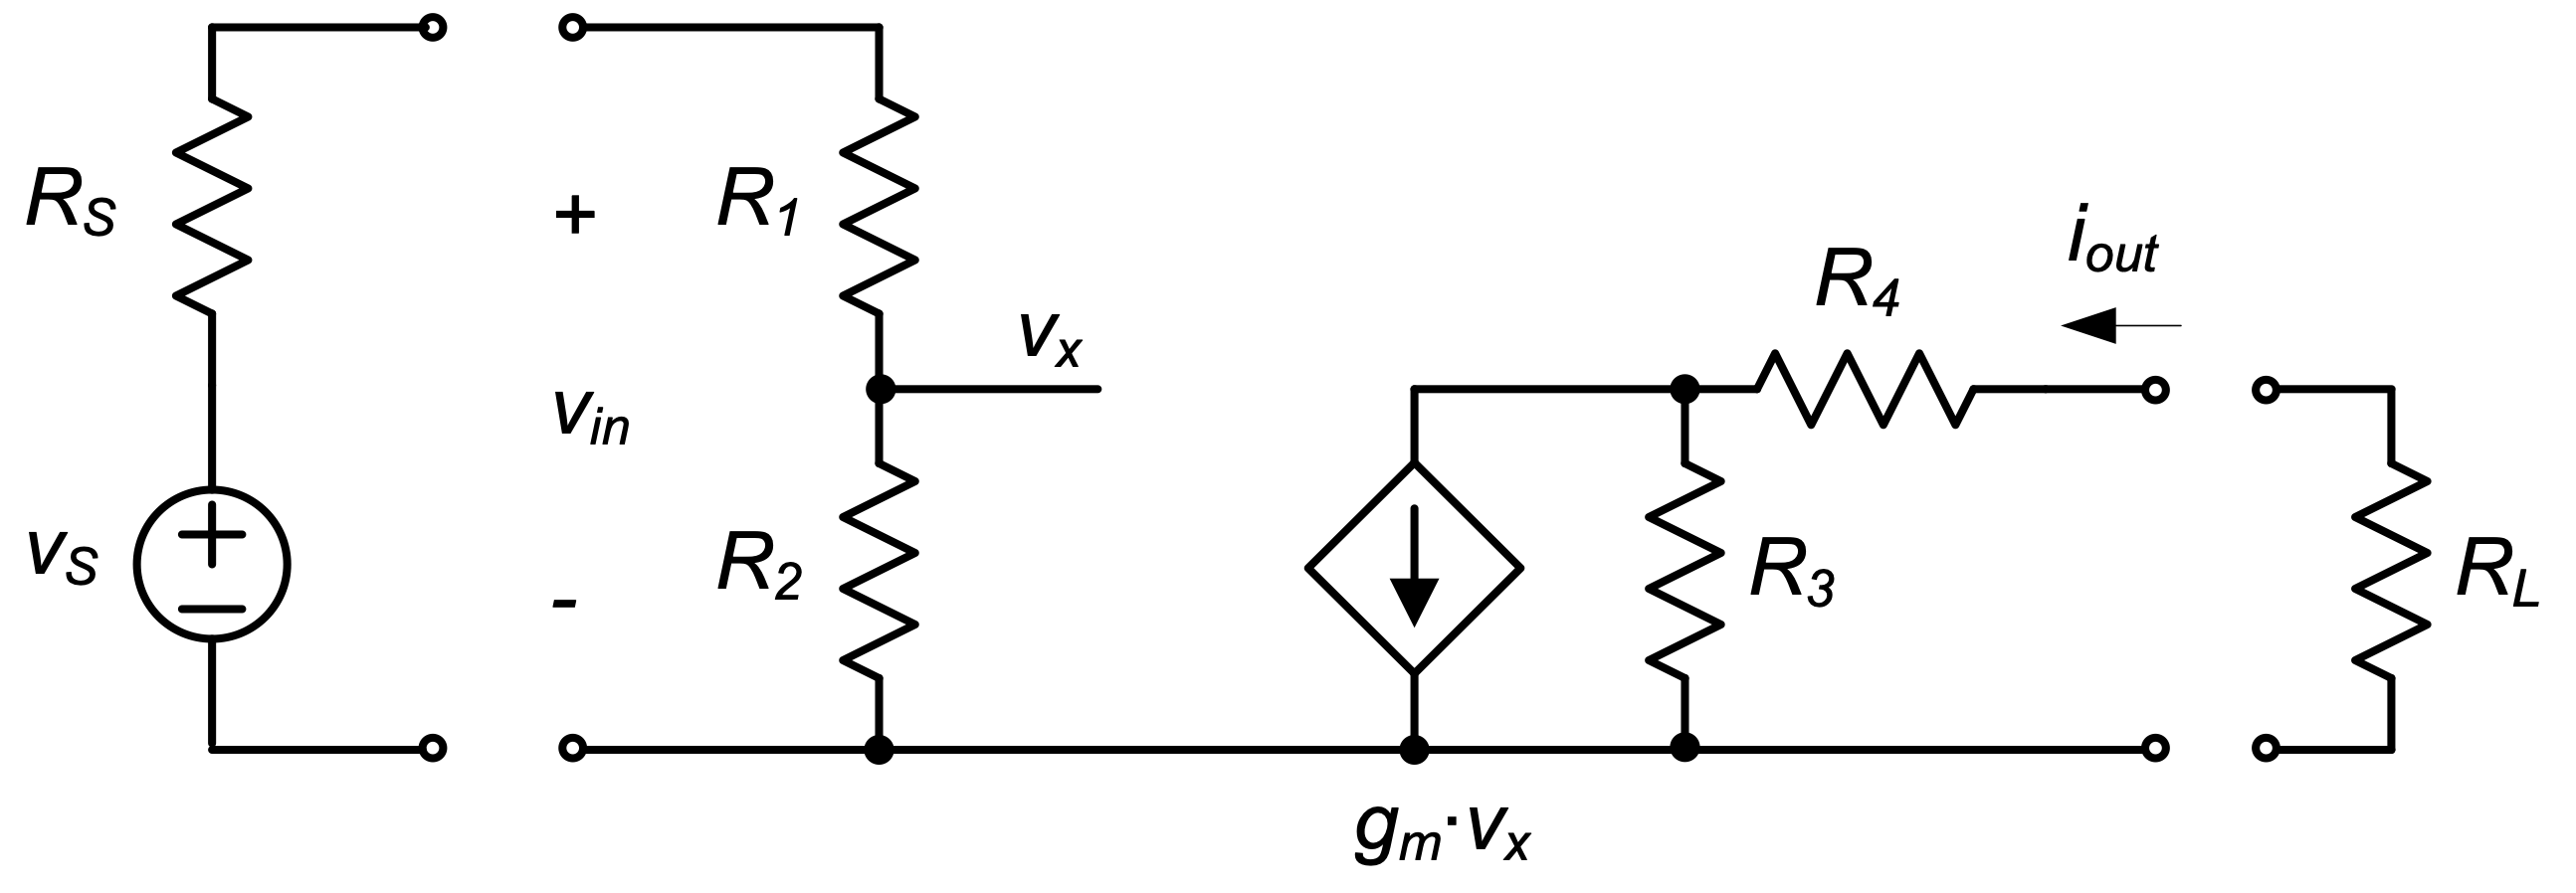
\includegraphics[width=0.5\textwidth,height=\textheight]{contents/chapter1/images/pdf/figure-ex-1.2a.pdf}

}

\caption{\label{fig-ex-1.2a}Figure Ex1-2A}

\end{figure}%

\textbf{SOLUTION}

To find the transconductance, we short the output port and apply an
ideal test voltage source (vt) at the input {[}see Figure Ex1-2B(a){]}.
From this circuit, we see that

\[
G_m = \frac{i_{sc}}{v_t} = \frac{g_m v_x \cdot \frac{R_3}{R_3 + R_4}}{v_t} = \frac{g_m v_x \cdot \frac{R_2}{R_1 + R_2} \cdot \frac{R_3}{R_3 + R_4}}{v_t} = g_m \cdot \frac{R_2}{R_1 + R_2} \cdot \frac{R_3}{R_3 + R_4}
\]

Next, to find Rin, we apply a test voltage at the input and connect the
load resistance RL at the output {[}Figure Ex1-2B(b){]}. From this
circuit, we find that the input resistance is simply the series
connection of R1 and R2, i.e., Rin = R1 + R2. Note that the output
network does not influence this result.

\begin{figure}

\centering{

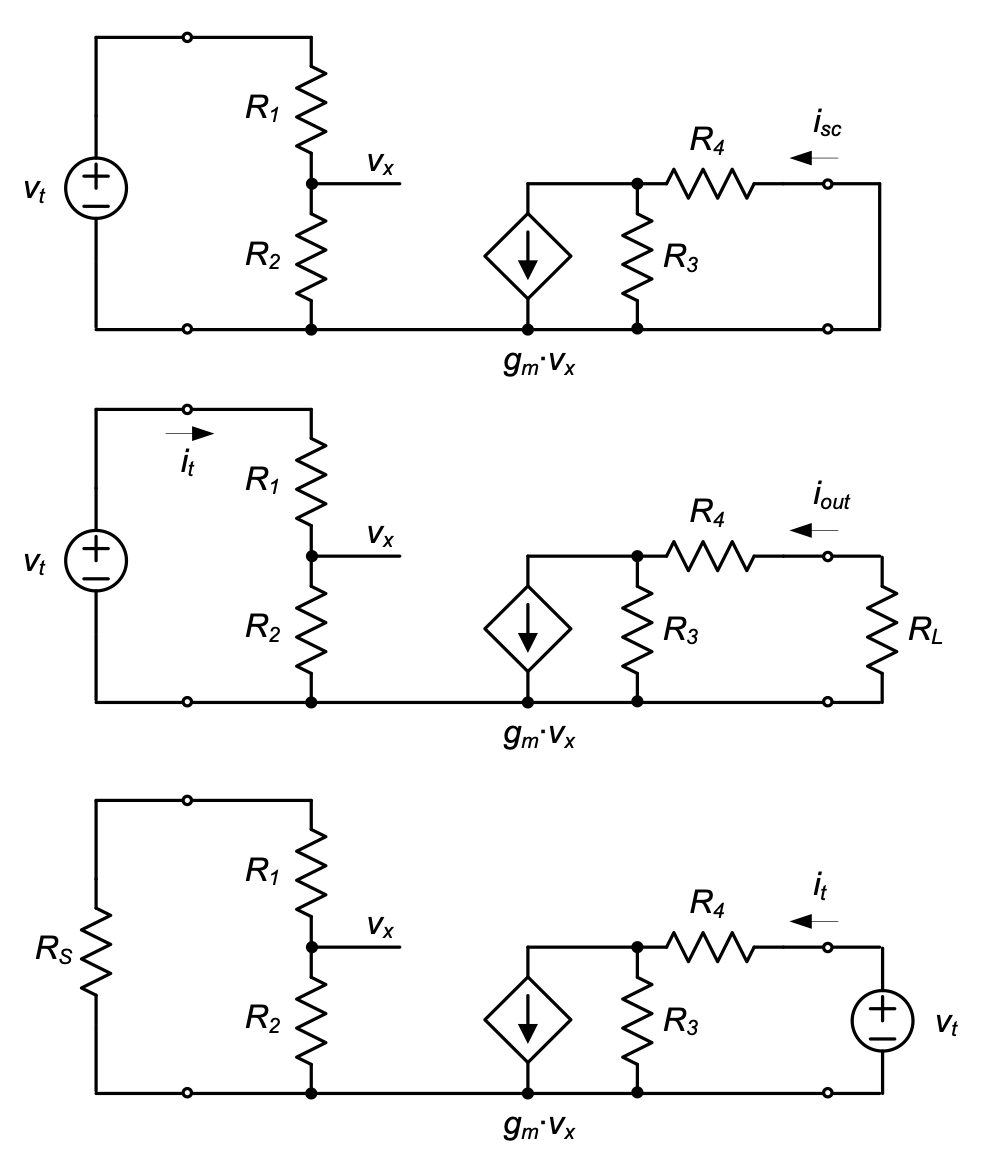
\includegraphics[width=0.5\textwidth,height=\textheight]{contents/chapter1/images/pdf/figure-ex-1.2b.pdf}

}

\caption{\label{fig-ex-1.2b}Figure Ex1-2B}

\end{figure}%

Finally, to find Rout, we apply a test voltage at the output and connect
the source resistance RS across the input port (the source vs is
replaced by a short), {[}see Figure Ex1-2B(c){]}. In the resulting
circuit, vx must be zero, because no current is flowing in the input
network. Thus, the controlled source carries no current and we conclude
that Rout = R3 + R4.

In order to compute the transfer function of the complete circuit, we
can reuse the result obtained in Example 1-1.

\[
G'_m = \frac{i_{out}}{v_s} = \Bigl(\frac{R_{in}}{R_{in} + R_s}\Bigr) \cdot G_m \cdot \Bigl(\frac{R_{L}}{R_{L} + R_{out}}\Bigr)
\]

Substituting Gm, Rin, and Rout from the above calcu- lation yields the
final result.

\[
G'_m = \frac{i_{out}}{v_s} = \frac{g_m R_2 R_3}{(R_1 + R_2 + R_S)(R_L + R_3 + R_4)}
\]

In the preceding example, we have seen that the source and load
resistances have no effect on the extracted two-port parameters. In the
following example, we will investigate a bilateral circuit to show that
in general, the input and output resistances depend on RS and RL, which
must therefore always be included in the general two-port modeling
calculations.

\textbf{Example 1-3: Two-Port Model Calculations for a Bilateral
Amplifier}

For the current amplifier in Figure Figure~\ref{fig-1.12}(a), calculate
the following unilateral two-port model parameters: the current gain Ai,
the input resistance Rin, and the output resistance Rout. Also, compute
the overall transfer function iout/vs using the obtained unilateral
two-port model. Compare the result to a direct KCL-based analysis of the
transfer function. Assume that the circuit is driven by a current source
with resistance RS and loaded by a resistance RL. For algebraic
simplicity, assume R1 = 1/gm (this case corresponds to the common-gate
amplifier circuit covered in Chapter 4).

\textbf{SOLUTION}

To find the current gain Ai, we short the output port and apply an ideal
test current source (it) at the input {[}see Figure Ex1-3(a){]}. From
this circuit, we see that

\[
v_{in} = \Bigl( g_m + \frac{1}{R_2} \Bigr)^{-1} \cdot i_t
\]

and

\[
i_{sc} = - \Bigl( g_m + \frac{1}{R_2} \Bigr) \cdot v_{in}
\]

Thus, Ai = isc/it = --1.

Next, to find Rin, we apply a test voltage at the input and connect the
load resistance RL at the output {[}Figure Ex1-3(b){]}. From this
circuit, we note that the input resistance is not easily identified by
inspection. Hence we write KCL for the two nodes of the circuit (vt and
vout).

\[
0 = -i_t + g_m v_t + \frac{v_t - v_out}{R_2}
\]

\[
0 = - g_m v_t + \frac{v_{out}}{R_L} + \frac{v_t - v_out}{R_2}
\]

Solving this system of equations yields

\[
R_{in} = \frac{v_t}{i_t} = \frac{R_2 + R_L}{1 + g_m R_2} = \frac{1 + \frac{R_L}{R_2}}{g_m + \frac{1}{R_2}}
\]

Note from this result that Rin depends on RL, as mentioned previously;
this dependency stems from the bilateral structure of the circuit. Also
note that Rin approaches 1/gm when R2 is large compared to RL and 1/gm.
We will revisit this important point in Chapter 4, in the context of a
common-gate amplifier circuit.

Figure Ex1-3 GOES HERE

Now, to find Rout, we apply a test voltage at the output and connect the
source resistance RS across the input port {[}Figure Ex1-3(c){]}. Again,
we must write KCL at the two circuit nodes and solve the resulting
system of equations. This yields

\[
R_{out} = \frac{v_t}{i_t} = R_2 R_S + g_m R_2 R_S
\]

Again, note that Rout is a function of RS; this is the case for any
bilateral circuit.

Finally, to compute the transfer function based on the obtained
unilateral model, we consider the circuit shown in Figure Ex1-3(d). By
inspection, we see that

\[
A_i' \frac{i_{out}}{i_s} = \Bigl( \frac{R_S}{R_{in} + R_S} \Bigr) A_i \frac{R_{out}}{R_L + R_{out}}
\]

Substituting Ai, Rin, and Rout from the above calcula- tion into this
expression yields

\[
A_{i, Two-Port}' = \frac{i_{out}}{i_s} = \frac{R_S(1 + g_m R_2)(R_2 + R_S + g_m R_2 R_S)}{(R_L + R_2 + R_S + g_m R_2 R_S)^2}
\]

We now wish to compare this result to the accurate transfer function of
the circuit, obtained by direct calculation and without approximating
the circuit as a unilateral two-port. For this purpose, we consider the
full circuit shown in Figure Ex1-3(e) and write KCL for its two nodes.

\[
0 = - i_s + g_m v_in + \frac{v_{in}}{R_S} + \frac{v_{in} - v_{out}}{R_2}
\]

\[
0 = -g_m v_{in} + \frac{v_{out}}{R_L} + \frac{v_{out} - v_{in}}{R_2}
\]

Solving this system of equations for vout and substi- tuting iout =
-vout/RL yields

\[
A_{i, Exact}' = \frac{i_{out}}{i_s} = \frac{i_{out}}{i_s} = 
\frac{R_S (1 + g_m R_2)}{R_L + R_2 + R_S + g_m R_2 R_S}
\]

The discrepancy factor between the two results is given by

\[
\frac{A_{i, Two-Port}'}{A_{i, Exact}'} = \frac{R_2 + R_S + g_m R_2 R_S}{R_L + R_2 + R_S + g_m R_2 R_S} = \frac{1 + R_S \Bigl(\frac{1}{R_2} + g_m}{1 + \frac{R_L}{R_2} + R_S \Bigl(\frac{1}{R_2} + g_m \Bigr)}
\]

From this result, we see that the discrepancy factor approaches unity
(nThe outcome of the above example captures the main spirit in which we
justify relying on unilateral two-port models in this module. Even
though the considered amplifier is strictly speaking bilateral, a
unilateral model describes its behavior to within the desired
engineering accuracy, provided that reasonable boundary conditions
hold.o error) when R2 is much larger than RL, a condition that is often
satisfied in practice (the ideal load for a current amplifier is a short
circuit). In this case, the unilateral two-port model will accurately
describe the behavior of the circuit.

The outcome of the above example captures the main spirit in which we
justify relying on unilateral two-port models in this module. Even
though the considered amplifier is strictly speaking bilateral, a
unilateral model describes its behavior to within the desired
engineering accuracy, provided that reason- able boundary conditions
hold.

\section{Integrated Circuit Design versus Printed Circuit Board
Design}\label{integrated-circuit-design-versus-printed-circuit-board-design}

In the design of analog circuits, the underlying technology has a
significant impact on the choice of architecture, because it tends to
restrict the availability and specification range of the underlying
active and passive components. For instance, a designer working with
discrete components on a printed circuit board may be subjected to the
following constraints:

\begin{itemize}
\item
  Limit the component count below 100 elements to achieve a small board
  area.
\item
  Resistors can be chosen in the range of 1Ω--10 MΩ.
\item
  Capacitors can be chosen in the range of 1 pF--10,000 μF.
\item
  The resistor and capacitor values match to within 1--10\%.
\item
  The available (discrete) bipolar junction transistors match to within
  20\% in their critical parameters.
\end{itemize}

In contrast, the designer of a CMOS system-on-chip may face the
constraints summarized below:

\begin{itemize}
\item
  Avoid using resistors; use as many MOSFET transistors as needed
  (within reasonable limits, on the order of hundreds to several
  thousands) to realize the best possible circuit implementation.
\item
  Capacitors can be chosen in the range of 10 fF--100 pF.
\item
  The critical parameters in the MOSFET transistors be made to match to
  within 1\%, but vary by more than 30\% for different fabrication runs.
\item
  Capacitors of similar size can match to within 0.1\%, but vary by more
  than 10\% for different fabrication runs.
\end{itemize}

As a consequence of the vastly different constraints that apply to the
design of analog circuits in CMOS technology, the resulting practical
and preferred circuit architectures differ substantially from the ones
that would be used in a printed circuit board design. For example, a
discrete voltage amplifier may utilize large AC coupling capacitors to
simplify and decouple the biasing of the individual gain stages (see
example in Figure 1-14). In contrast, it is typically not possible to
use AC coupling techniques (except for very high-frequency designs) in
integrated circuits, primarily due to the restriction on maximum
capacitor size.

INSERT FIGURE 14 HERE

The material covered in this module is primarily concerned with analog
integrated circuit design. While this choice does not affect many of the
key principles used in the analysis and the discussed circuits, it does
affect the architectural choices made in arriving at a practical design.
For instance, large AC coupling capacitors are not used throughout the
discussion. Also, where appropriate, we will invoke certain assumptions
about the typical matching of component parameters in CMOS to eliminate
impractical design choices.

\section{Prerequisites and Advanced
Material}\label{prerequisites-and-advanced-material}

The reader of this module is expected to be familiar with the basis
concepts of linear circuit analysis (see Refer- ence 3), including

\begin{itemize}
\item
  Passive components (resistors, capacitors)
\item
  Kirchhoff's voltage and current laws (KVL and KCL)
\item
  Independent and dependent voltage and current sources; Thevénin and
  Norton representation of controlled sources
\item
  Two-port representation of circuits; calculation of port resistances
  and frequency dependent imped- ances
\item
  Manipulation of complex variables and numbers
\item
  Phasor analysis and Laplace domain representa- tion of passive circuit
  elements
\item
  Bode plots
\end{itemize}

The derivations of device models in this module assume familiarity with
basic solid-state physics and electrostatics as treated in introductory
texts on solid-state device physics (see Reference 4). A few sections of
this module are marked with an asterisk (*) to indicate advanced
material that may in some cases go beyond the learning goals of an
introductory course. These sections can be skipped at the instructor's
discretion without affecting the overall flow and context.

\section{Notation}\label{notation}

This module follows the notation for signal variables as standardized by
the IEEE. Total signals are composed of the sum of DC quantities and
small signals. For example, a total input voltage vIN is the sum of a DC
input voltage VIN and a small-signal voltage vin. The notation is
summarized below.

\begin{itemize}
\item
  Total quantity has a lowercase variable name and uppercase subscript
\item
  DC quantity has an uppercase variable name and uppercase subscript
\item
  Small-signal quantity has a lowercase variable name and lowercase
  subscript
\end{itemize}

\chapter{Summary}\label{summary}

This chapter offered a brief motivation for the topics covered in this
module, which focuses on the analysis and design of elementary amplifier
stages in CMOS technology. These elementary stages can be viewed as the
``atoms'' of analog circuit design and a thorough understanding of the
blocks is a necessary prerequisite for the design of advanced analog
circuits design, as for instance in the context of large
systems-on-chip. At all levels of circuit design, complexity is managed
using hierarchical abstraction and model simplification using proper
engineering approximations. The unilateral two-port models reviewed in
Section 1-3 and used throughout this module, are an example of such
abstractions.

INSERT Figure P1-1 HERE

\chapter{Problems}\label{problems}

\textbf{P1.1} Given the amplifier circuit in Figure P1-1 (a) Find the
input and output resistance. (b) Construct an equivalent circuit using a
voltage amplifier two-port model and determine all model parameters
symbolically. (c) Repeat part (b) for a current amplifier model. (d)
Repeat part (b) for a transconductance amplifier model. (e) Repeat part
(b) for a transresistance amplifier model.

\textbf{P1.2} Convince yourself that the circuits of Figure 1-10 and
Figure 1-11 are equivalent by showing sym- bolically that both circuits
have the same overall voltage gain A′v = v out ⁄ v s .

\textbf{P1.3} You are given an input voltage source with a source
resistance, RS. (a) Use the unilateral voltage amplifier two-port model
found in P1.1 to find the overall voltage gain when the amplifier is
driving a load resistor RL . (b) Specify whether the resistances r1, ri,
ro, r2 in the small signal model should be increased, be decreased, or
remain the same to improve the overall voltage gain.

\textbf{P1.4} You are given an input current source with a source
resistance, RS. (a) Use the unilateral current amplifier two-port model
found in P1.1 to find the overall current gain when the amplifier is
driving a load resistor RL . (b) Specify whether the resistances r1, ri,
ro, r2 in the small-signal model should be increased, be decreased, or
remain the same to improve the overall current gain.

\textbf{P1.5} Given the circuit model in Figure P1-5 for an amplifier
circuit (a) Find the input and output resistance. (b) Construct a
two-port model for a unilateral voltage amplifier. (c) Construct a
two-port model for a unilateral current amplifier. (d) Construct a
two-port model for a unilateral transconductance amplifier. (e)
Construct a two-port model for a unilateral transresistance amplifier.

INSERT Figure P1-5 HERE

\textbf{P1.6} Consider the two-port model of a voltage amplifier as
shown in Figure 1-9(a) with the following parameters: Av = 10, Rin = 5
kΩ, and Rout = 100 Ω.

\begin{enumerate}
\def\labelenumi{(\alph{enumi})}
\tightlist
\item
  Draw the two-port model for a transresistance amplifier by conversion
  from the voltage amplifier model.
\item
  Draw the two-port model for a transconductance amplifier by conversion
  from the voltage amplifier model.
\item
  Draw the two-port model for a current amplifier by conversion from the
  voltage amplifier model.
\end{enumerate}

\textbf{P1.7} Derive an expression for the transresistance vout/iin for
the circuit of Figure 1-7 using the following parameters: Ai1 = 1, Gm2 =
10 mS, Av3 = 0.8, Rin1 = 50 Ω, Rout1 = 500 Ω, Rout2 = 1 kΩ, and Rout3 =
100 Ω. Using this result, lump the entire circuit into a single
transresistance amplifier as shown in Figure 1-9(d). Draw the resulting
model, including Rin and Rout.

\textbf{P1.8} Consider the amplifier circuit of Figure 1-12(a) with R1 =
1/gm = 1 kΩ and R2 = 100 kΩ. Compute all component values for the
bilateral two-port current amplifier model of Figure 1-12(b). Note that
Aif, Rin, and Rout can be described as explained in Section 1-3. Similar
to Aif, Air is found by short-circuiting the input port and by injecting
a test current into the output port. Compare the relative magnitude of
Aif and Air.

\chapter{Transfer Characteristic of the Common-Source Voltage
Amplifier}\label{sec-dl_primer}

(\citeproc{ref-rosenblatt1957perceptron}{Rosenblatt 1957}), followed by
the invention of backpropagation algorithms in the 1980s
(\citeproc{ref-rumelhart1986learning}{Rumelhart, Hinton, and Williams
1986}).

\part{REFERENCES}

\chapter*{References}\label{references-1}
\addcontentsline{toc}{chapter}{References}

\markboth{References}{References}

\phantomsection\label{refs}
\begin{CSLReferences}{1}{0}
\bibitem[\citeproctext]{ref-rosenblatt1957perceptron}
Rosenblatt, Frank. 1957. \emph{The Perceptron, a Perceiving and
Recognizing Automaton Project Para}. Cornell Aeronautical Laboratory.

\bibitem[\citeproctext]{ref-rumelhart1986learning}
Rumelhart, David E., Geoffrey E. Hinton, and Ronald J. Williams. 1986.
{``Learning Representations by Back-Propagating Errors.''} \emph{Nature}
323 (6088): 533--36. \url{https://doi.org/10.1038/323533a0}.

\end{CSLReferences}


\backmatter


\end{document}
